% ju 18-Feb-24 Hardware.tex
\documentclass{vorlage-design-main}
\usepackage[utf8]{inputenc}
\usepackage{longtable}
\usepackage{blindtext,alltt}
%% Ganze Überschrift
\title{Thema}

%% Kürzerer Titel zur Verwendung im Seitenkopf
\runningtitle{Kurztitel}
\author{Jan Unger}
% \author{2.}
\date{\today}

%% Die .bib-Datei mit vollständigen Referenzen zur Verwendung mit biblatex. articleclass lädt das Paket biblatex-chicago mit Anpassungen
\addbibresource{literatur.bib}

\begin{document}

\maketitle

\begin{abstract}

\end{abstract}

\hypertarget{arduino-uno-r3-board}{%
\subsection{Arduino Uno R3 Board}\label{arduino-uno-r3-board}}

\begin{figure}
\centering
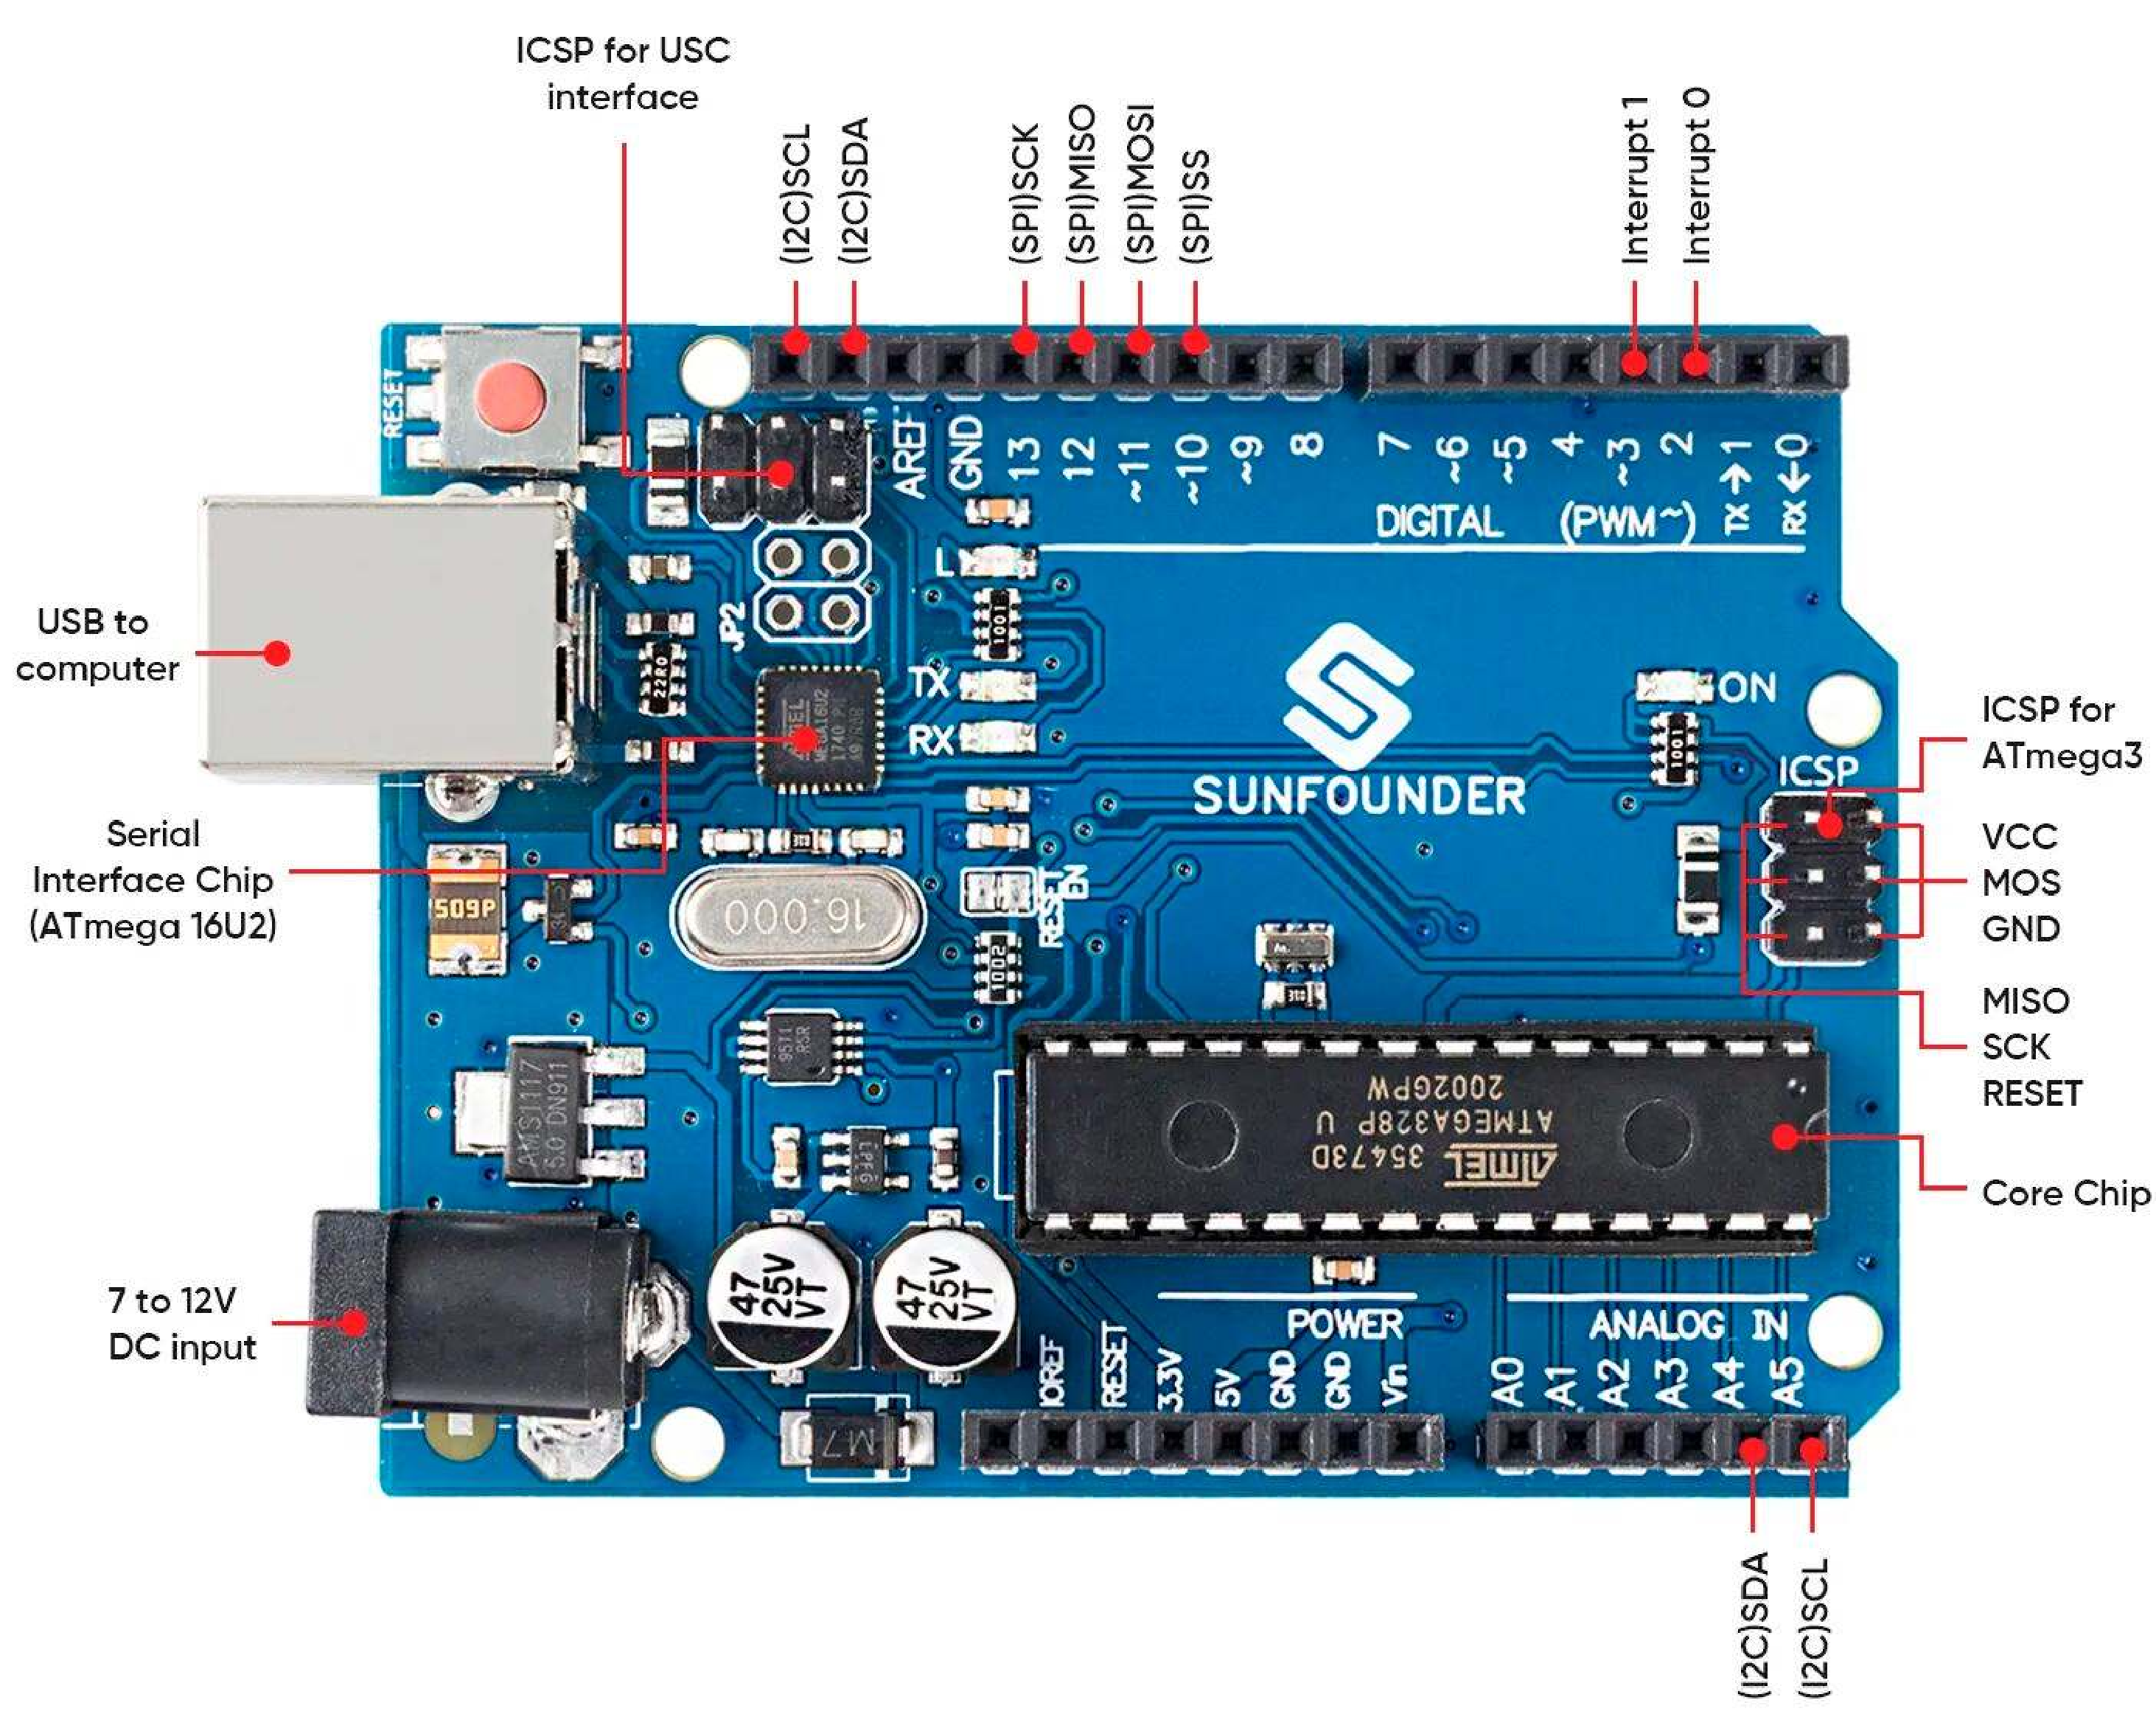
\includegraphics[width=0.8\textwidth]{images/uno.pdf}
\floatnotes{}
%\label{fig:}
\caption{Arduino Uno}
\end{figure}

\begin{itemize}

\item
  \textbf{Mikrocontroller}: ATmega328P, Herz des Arduino Uno R3 Boards,
  ermöglicht die Steuerung und Verarbeitung von Daten.
\item
  \textbf{Betriebsspannung}: 5V, standardmäßig für die meisten
  elektronischen Komponenten und Sensoren geeignet.
\item
  \textbf{Eingangsspannung}:

  \begin{itemize}
  
  \item
    Empfohlen: 7-12V, idealer Bereich für stabile Leistung.
  \item
    Limit: 6-20V, maximal zulässiger Bereich, wobei Spannungen über 12V
    das Board beschädigen können.
  \end{itemize}
\item
  \textbf{Digitale I/O-Pins}: 14 (mit den Nummern 0-13), von denen 6
  Pins (3, 5, 6, 9-11) für PWM-Ausgänge genutzt werden können, erlauben
  eine flexible Steuerung von Elektronik.
\item
  \textbf{Analoge Eingangspins}: 6 (A0-A5), für die Erfassung von
  analogen Signalen wie von Sensoren.
\item
  \textbf{DC Strom pro I/O-Pin}: 20 mA, gibt den maximalen Stromfluss
  pro Pin an.
\item
  \textbf{DC Strom für 3.3V Pin}: 50 mA, maximaler Stromfluss für den
  3.3V Spannungsausgang.
\item
  \textbf{Speicher}:

  \begin{itemize}
  
  \item
    \textbf{Flash-Speicher}: 32 KB, für den Programmcode, wobei 0,5 KB
    vom Bootloader belegt werden.
  \item
    \textbf{SRAM}: 2 KB, für Variablen während der Programmausführung.
  \item
    \textbf{EEPROM}: 1 KB, für dauerhafte Datenspeicherung über
    Neustarts hinweg.
  \end{itemize}
\item
  \textbf{Taktfrequenz}: 16 MHz, bestimmt die Geschwindigkeit der
  Programmausführung.
\item
  \textbf{LED\_BUILTIN}: Pin 13, häufig verwendet für Testzwecke oder
  als einfache Statusanzeige.
\item
  \textbf{Physische Abmessungen}:

  \begin{itemize}
  
  \item
    Länge: 68,6 mm
  \item
    Breite: 53,4 mm
  \item
    Gewicht: 25 g
  \end{itemize}
\item
  \textbf{I2C-Port}: A4 (SDA) und A5 (SCL), für die Kommunikation mit
  I2C-kompatiblen Geräten.
\end{itemize}

\hypertarget{flash-speicher-32-kb}{%
\subsubsection{FLASH-SPEICHER: 32 KB}\label{flash-speicher-32-kb}}

\begin{itemize}

\item
  \textbf{Verwendung}: Der Flash-Speicher dient zur Speicherung des
  Programmcodes. Mit 32 KB Speicherplatz können relativ umfangreiche
  Programme auf den ATmega328P geladen werden.
\item
  \textbf{Bootloader}: Ein kleiner Teil des Flash-Speichers, 0,5 KB, ist
  für den Bootloader reserviert. Der Bootloader ermöglicht das
  Programmieren des Mikrocontrollers über eine einfache serielle
  Schnittstelle, ohne dass ein externes Programmiergerät erforderlich
  ist. Dies erleichtert das Hochladen von Programmen erheblich.
\end{itemize}

\hypertarget{sram-2-kb}{%
\subsubsection{SRAM: 2 KB}\label{sram-2-kb}}

\begin{itemize}

\item
  \textbf{Verwendung}: SRAM (Static Random-Access Memory) wird für die
  Speicherung von Variablen und Zwischenergebnissen während der
  Ausführung eines Programms verwendet. Mit 2 KB bietet der ATmega328P
  genügend Platz für die meisten Anwendungen, die nicht extrem
  speicherintensiv sind.
\item
  \textbf{Eigenschaften}: SRAM ist flüchtig, d.h., die Daten gehen
  verloren, wenn die Stromversorgung unterbrochen wird. Es ist jedoch
  schnell und ermöglicht einen effizienten Zugriff während der Laufzeit
  des Programms.
\end{itemize}

\hypertarget{eeprom-1-kb}{%
\subsubsection{EEPROM: 1 KB}\label{eeprom-1-kb}}

\begin{itemize}

\item
  \textbf{Verwendung}: EEPROM (Electrically Erasable Programmable
  Read-Only Memory) dient zur dauerhaften Speicherung von Daten. Im
  Gegensatz zu Flash und SRAM bleiben die im EEPROM gespeicherten Daten
  auch nach dem Ausschalten des Mikrocontrollers erhalten.
\item
  \textbf{Eigenschaften}: Mit 1 KB Speicherplatz bietet das EEPROM Platz
  für Konfigurationsdaten, Kalibrierwerte oder kleine Datenmengen, die
  zwischen den Neustarts des Mikrocontrollers persistent bleiben müssen.
  EEPROM-Zugriffe sind in der Regel langsamer als Flash- oder
  SRAM-Zugriffe und haben eine begrenzte Anzahl von
  Schreib-/Löschzyklen.
\end{itemize}

\hypertarget{galaxyrvr-shield}{%
\subsection{GalaxyRVR Shield}\label{galaxyrvr-shield}}

\begin{figure}
\centering
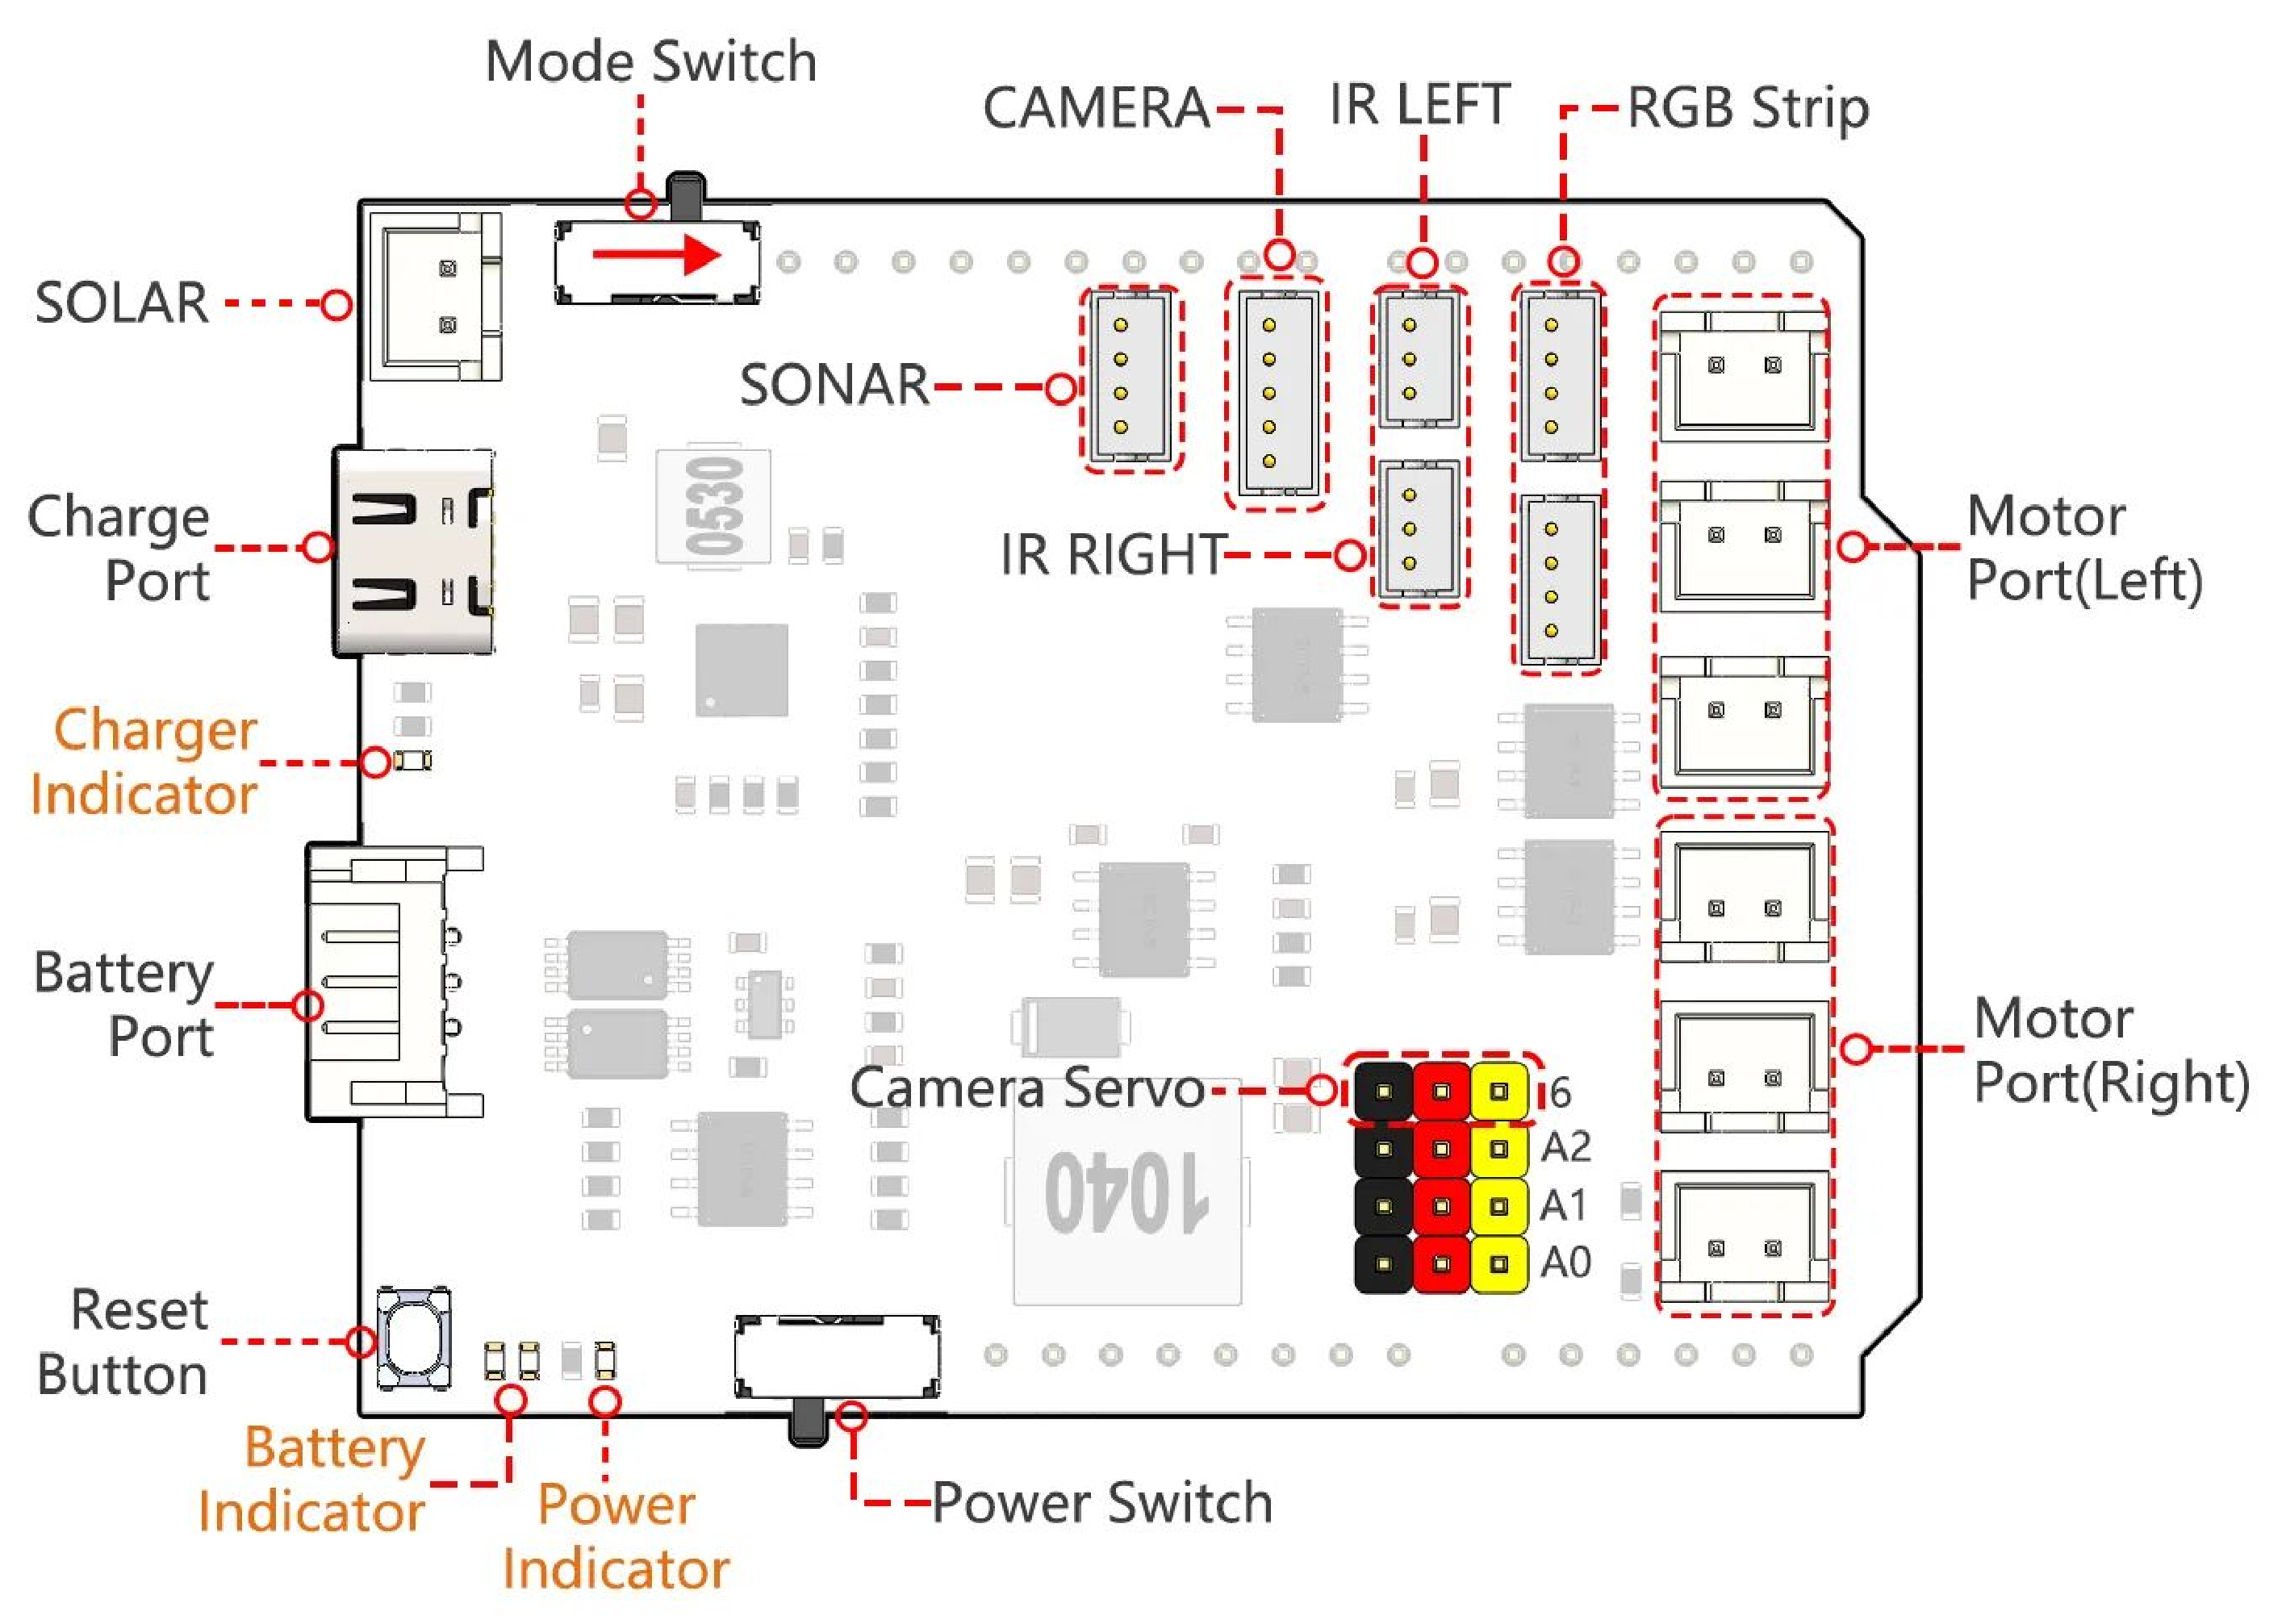
\includegraphics[width=0.8\textwidth]{images/galaxyrvr_shield_pinout.pdf}
\floatnotes{}
%\label{fig:}
\caption{GalaxyRVR Shield Pinbelegung}
\end{figure}

\begin{itemize}

\item
  \textbf{Allgemeine Merkmale}:

  \begin{itemize}
  
  \item
    Basierend auf dem ATmega328P Mikrocontroller.
  \item
    Bietet 14 digitale Ein-/Ausgangspins, 6 analoge Eingänge und 6
    PWM-Ausgänge.
  \item
    Enthält einen 16 MHz Keramikresonator, USB-Verbindung, Strombuchse,
    ICSP-Header, Reset-Knopf.
  \end{itemize}
\item
  \textbf{Stromversorgung}:

  \begin{itemize}
  
  \item
    Betriebsspannung: 5V.
  \item
    Empfohlene Eingangsspannung: 7-12V.
  \item
    Grenzwert der Eingangsspannung: 6-20V.
  \item
    Integrierter Ladekreislauf für Akkus mit PH2.0-3P Schnittstelle,
    geschätzte Ladezeit: 130 Minuten.
  \end{itemize}
\item
  \textbf{Spezifische Funktionen}:

  \begin{itemize}
  
  \item
    \textbf{Motoranschlüsse}: Zwei Sets für Motoranschlüsse erlauben den
    Anschluss von bis zu 6 Motoren, gesteuert durch Signalpins 2, 3
    (rechts) und 4, 5 (links).
  \item
    \textbf{RGB-Streifen}: Anschlüsse für 2 RGB-LED-Streifen, verbunden
    mit Pins 12, 13 und 11.
  \item
    \textbf{IR-Hindernisvermeidung}: Anschlüsse für links und rechts
    IR-Hindernisvermeidungsmodule, angeschlossen an Pins 8 und 7.
  \item
    \textbf{Kamera}: Anschluss für Kamera-Adapter-Board, unterstützt
    ESP32 CAM.
  \item
    \textbf{Ultraschallmodul}: Anschluss für das Ultraschallmodul, Trig-
    und Echo-Pins sind an Pin 10 angeschlossen.
  \item
    \textbf{Solarpanelanschluss}: Ermöglicht das Laden des Akkus über
    Solarpanel.
  \end{itemize}
\item
  \textbf{Weitere Features}:

  \begin{itemize}
  
  \item
    \textbf{Ladeanzeige}: Rote LED signalisiert das Laden über
    USB-C-Port.
  \item
    \textbf{Betriebsanzeige}: Grüne LED zeigt den Betriebsstatus an.
  \item
    \textbf{Batterieanzeige}: Zwei orangefarbene LEDs zeigen den
    Batteriestatus an.
  \item
    \textbf{Reset-Knopf}: Ermöglicht das Zurücksetzen des Programms auf
    dem Arduino-Board.
  \item
    \textbf{Netzschalter}: Zum Ein- und Ausschalten des GalaxyRVR
    Shields.
  \item
    \textbf{Modus-Schalter}: Für die Nutzung des ESP32-CAM; Änderung der
    Position notwendig beim Hochladen von Code, um Konflikte zu
    vermeiden.
  \end{itemize}
\end{itemize}

\hypertarget{esp32-cam-modul}{%
\subsection{ESP32-CAM Modul}\label{esp32-cam-modul}}

\begin{figure}
\centering
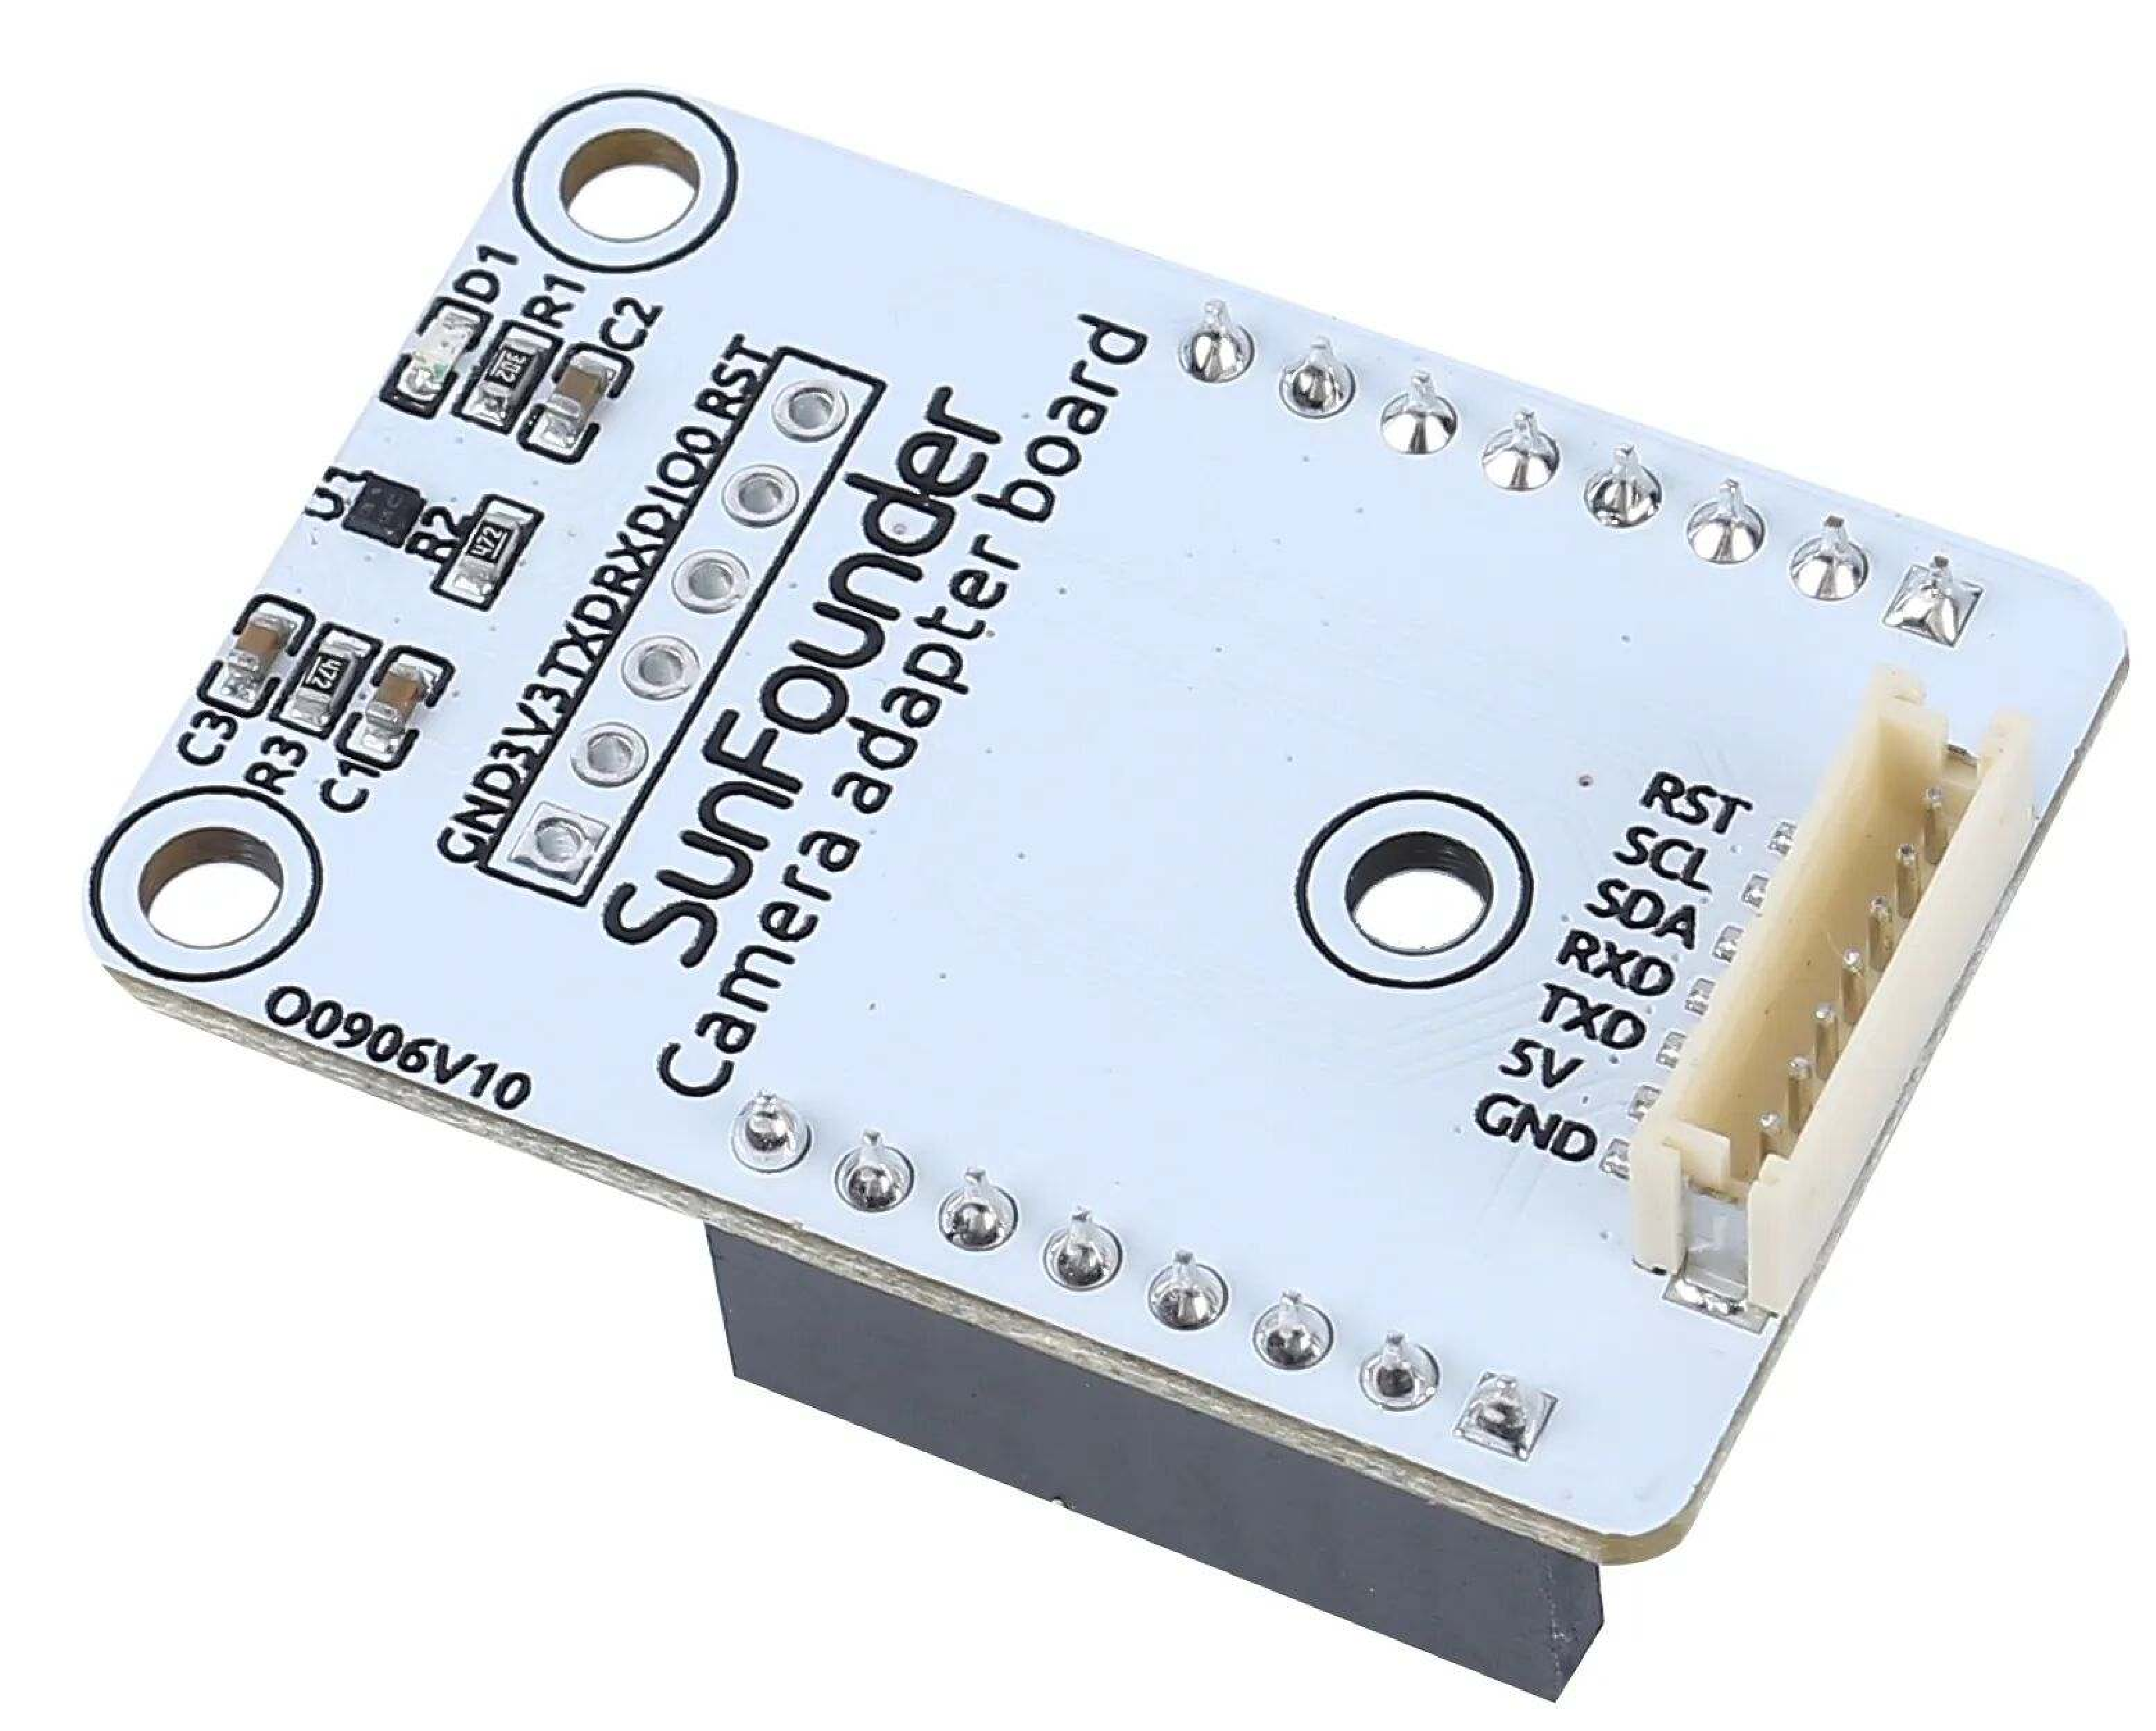
\includegraphics[width=0.8\textwidth]{images/cam_adapter_board.pdf}
\floatnotes{}
%\label{fig:}
\caption{Kameraadapter-Board}
\end{figure}

\hypertarget{kernmerkmale-des-esp32-cam}{%
\subsubsection{Kernmerkmale des
ESP32-CAM}\label{kernmerkmale-des-esp32-cam}}

\begin{itemize}

\item
  \textbf{Preis}: Ungefähr 10 Dollar, macht es zu einer erschwinglichen
  Option für verschiedene Projekte.
\item
  \textbf{Kompakte Größe}: Mit Abmessungen von nur 27x40.5x4.5mm ist es
  extrem platzsparend.
\item
  \textbf{Geringer Stromverbrauch}: Im Tiefschlafmodus verbraucht das
  Modul nur 6mA, was es besonders energieeffizient macht.
\end{itemize}

\hypertarget{technische-spezifikationen}{%
\subsubsection{Technische
Spezifikationen}\label{technische-spezifikationen}}

\begin{itemize}

\item
  \textbf{Mikrocontroller}: ESP32-S, unterstützt durch 520KB internes
  RAM und zusätzlich 8MB externes PSRAM.
\item
  \textbf{Kamera}: OV2640 Kamera integriert.
\item
  \textbf{Kommunikation}: Unterstützt Wi-Fi 802.11 b/g/n/e/i und
  Bluetooth 4.2 BR/EDR sowie BLE-Standards.
\item
  \textbf{Speicher}: Standardmäßig mit 32Mbit SPI Flash ausgestattet.
\item
  \textbf{Schnittstellen}: Bietet UART, SPI, I2C, PWM und unterstützt
  microSD-Karten bis zu 4G.
\item
  \textbf{IO Pins}: Verfügt über 9 nutzbare GPIO Pins.
\item
  \textbf{Stromversorgung}: Kann über einen 4.75-5.25V Eingang versorgt
  werden.
\end{itemize}

\hypertarget{pinbelegung-des-esp32-cam-ai-thinker-modul}{%
\subsubsection{Pinbelegung des ESP32-CAM (AI-Thinker
Modul)}\label{pinbelegung-des-esp32-cam-ai-thinker-modul}}

\begin{figure}
\centering
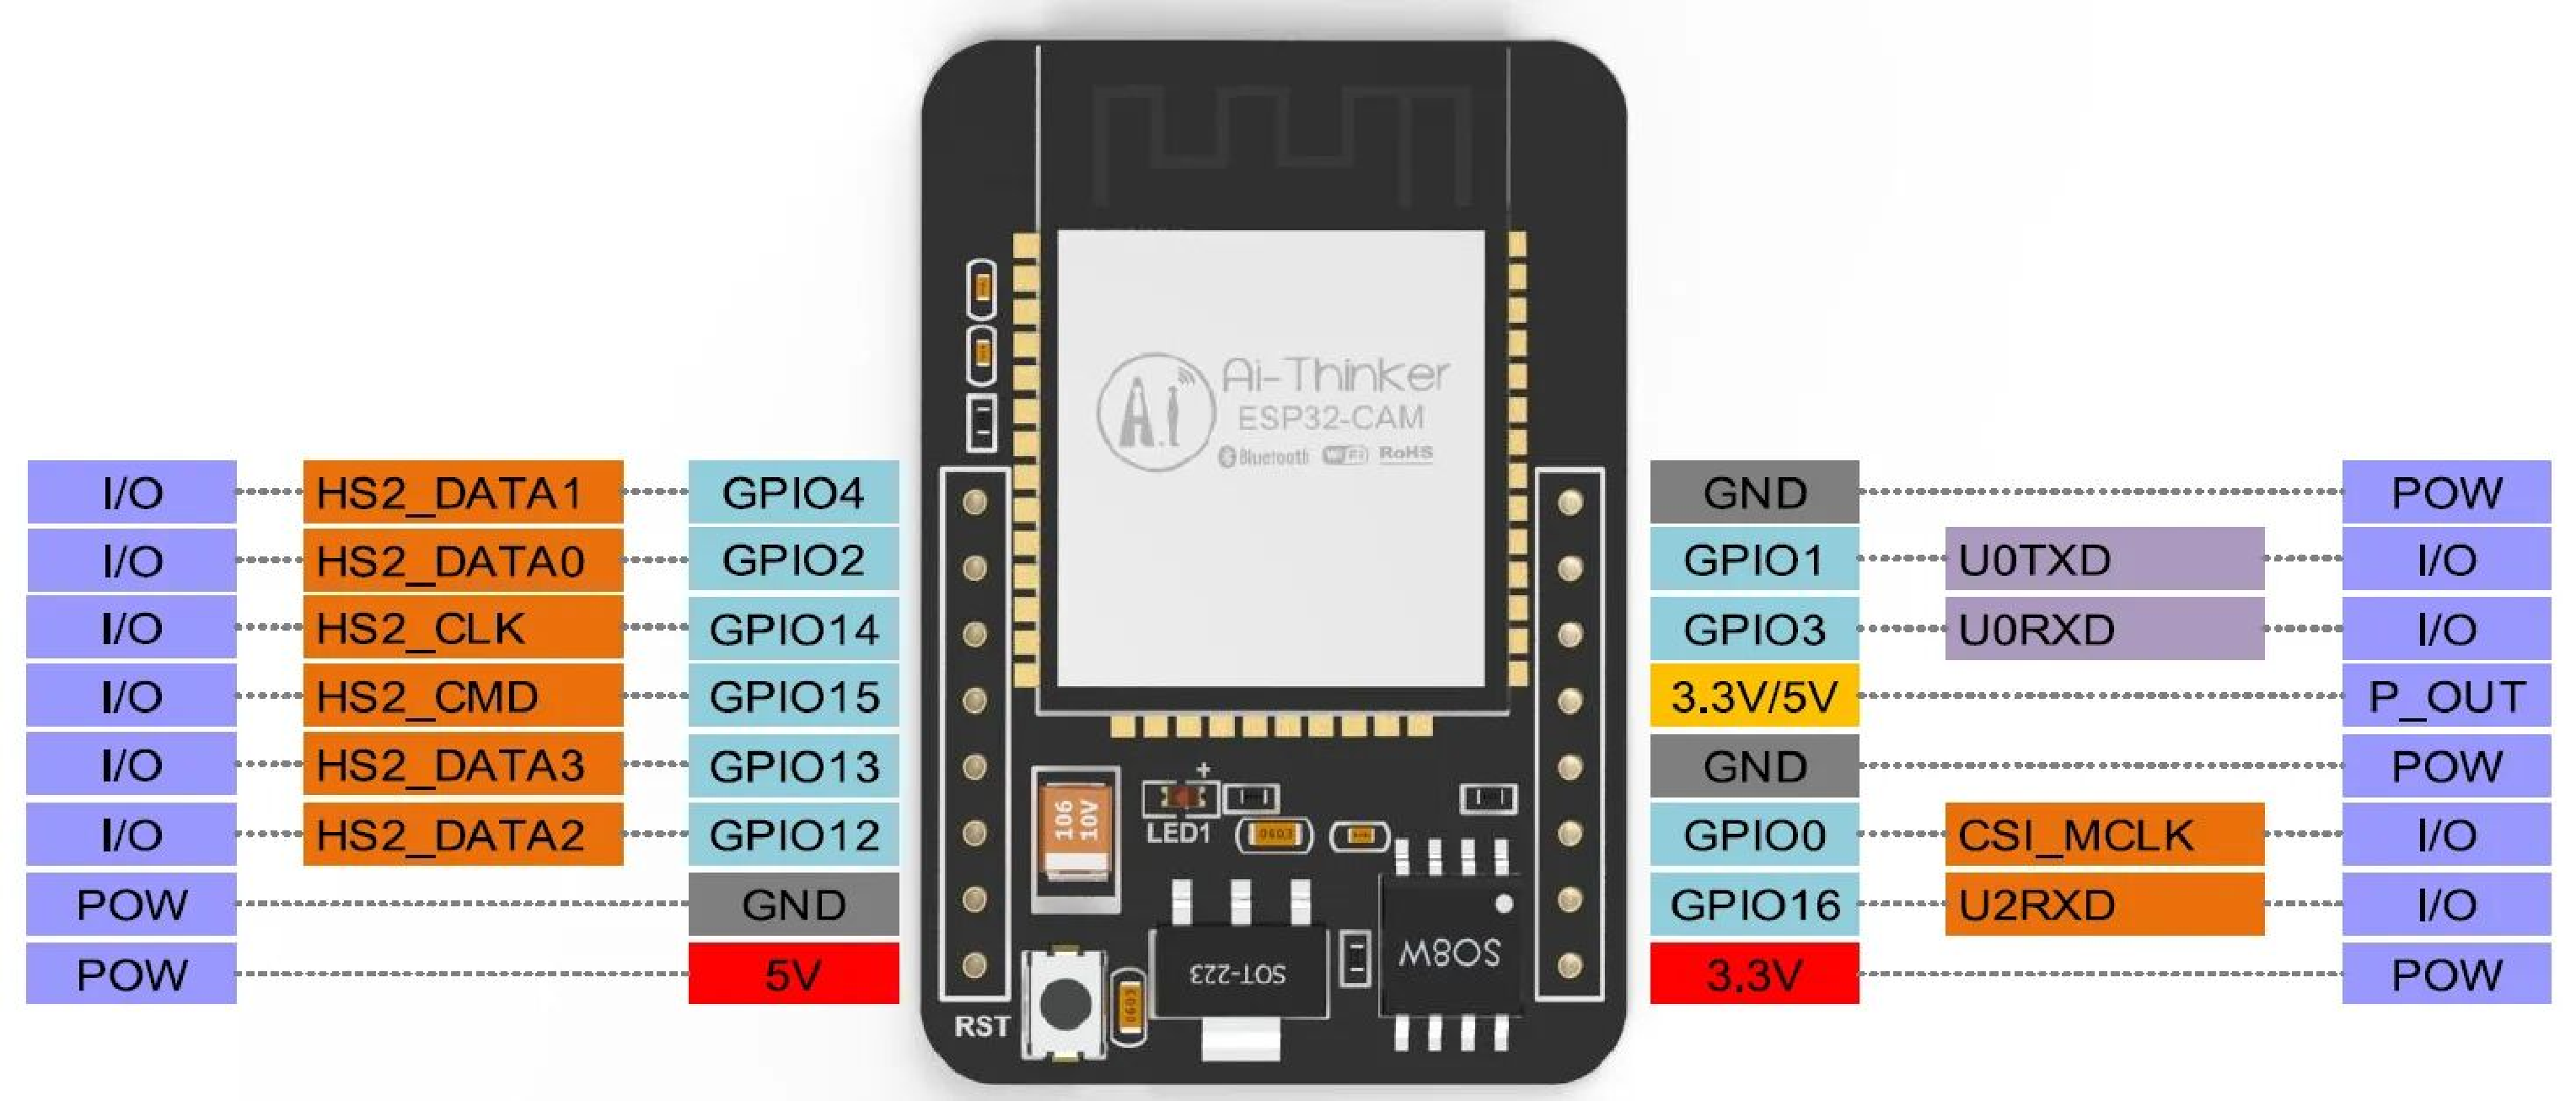
\includegraphics[width=0.8\textwidth]{images/esp32_cam_pinout.pdf}
\floatnotes{}
%\label{fig:}
\caption{ESP32-CAM Pinbelegung}
\end{figure}

\begin{itemize}

\item
  \textbf{Stromversorgung und Erdung}:

  \begin{itemize}
  
  \item
    Drei GND-Pins für die Erdung.
  \item
    Drei Pins für die Stromversorgung: 3.3V, 5V und ein wählbarer Pin
    für entweder 3.3V oder 5V.
  \end{itemize}
\item
  \textbf{Serielle Kommunikation}:

  \begin{itemize}
  
  \item
    GPIO 1 und GPIO 3 dienen als serielle Pins, notwendig für das
    Hochladen von Code auf das Board.
  \end{itemize}
\item
  \textbf{Flash-Modus}:

  \begin{itemize}
  
  \item
    GPIO 0 entscheidet über den Flash-Modus des ESP32. Bei Verbindung
    von GPIO 0 mit GND tritt der ESP32 in den Flash-Modus.
  \end{itemize}
\item
  \textbf{Anschluss des microSD-Kartenlesers}:

  \begin{itemize}
  
  \item
    GPIO 14 (CLK), GPIO 15 (CMD), GPIO 2 (Daten 0), GPIO 4 (Daten 1 und
    an Bord LED), GPIO 12 (Daten 2), GPIO 13 (Daten 3) sind mit dem
    microSD-Kartenleser verbunden.
  \end{itemize}
\end{itemize}

\hypertarget{einsatzgebiete}{%
\subsubsection{Einsatzgebiete}\label{einsatzgebiete}}

Das ESP32-CAM Modul eignet sich hervorragend für eine Vielzahl von
IoT-Anwendungen, darunter:

\begin{itemize}

\item
  Heim-Smart-Geräte
\item
  Industrielle drahtlose Steuerung
\item
  Drahtlose Überwachung
\item
  QR-drahtlose Identifikation
\item
  Drahtlose Positionierungssysteme
\end{itemize}

\hypertarget{hinweise-zur-verwendung}{%
\subsubsection{Hinweise zur Verwendung}\label{hinweise-zur-verwendung}}

\begin{itemize}

\item
  \textbf{Stromversorgung}: Für eine optimale Funktion sollte das Modul
  mit mindestens 5V und 2A versorgt werden.
\item
  \textbf{GPIO32}: Steuert die Stromversorgung der Kamera. Muss für den
  Betrieb nach unten gezogen werden.
\item
  \textbf{GPIO0}: Wichtig für den Flash-Modus des ESP32. Muss mit GND
  verbunden sein, um den Flash-Modus zu aktivieren.
\item
  \textbf{Interne Anschlüsse}: Mehrere GPIOs sind intern mit dem
  microSD-Kartenleser verbunden, was bei der Verwendung dieser Pins
  berücksichtigt werden muss.
\end{itemize}

\begin{table}[!ht]
\caption{}% \label{tab:}%% anpassen
\begin{tabular}{@{}ll@{}}

\toprule
Merkmal & Spezifikation \\
\midrule[\heavyrulewidth]

Modell & ESP32-CAM \\
Gehäuse & DIP-16 \\
Größe & 27*40.5*4.5(+/-0.2)mm \\
SPI Flash & Standard 32Mbit \\
RAM & Intern 520KB + Extern 8MB PSRAM \\
Bluetooth & Bluetooth 4.2 BR/EDR und BLE-Standards \\
Wi-Fi & 802.11 b/g/n/e/i \\
Unterstützte Schnittstellen & UART, SPI, I2C, PWM \\
Unterstützt TF-Karte & bis zu 4G \\
IO Pins & 9 \\
Serielle Portgeschwindigkeit & Standard 115200 bps \\
Bildausgabeformat & JPEG (nur OV2640 unterstützt), BMP, GRAUSTUFE \\
Spektrumbereich & 2400 \textasciitilde2483.5MHz \\
Antennentyp & On-Board PCB-Antenne, Gewinn 2dBi \\
Sendeleistung & 802.11n: 13+/-2 dBm (@MCS7) \\
Empfindlichkeit & CCK, 1 Mbps: -90dBm \\
Stromverbrauch & Tiefschlaf: 6mA@5V \\
Sicherheit & WPA/WPA2/WPA2-Enterprise/WPS \\
Stromversorgungsbereich & 4.75-5.25V \\
Betriebstemperatur & -20 \textasciitilde{} 70 °C \\
Lagerumgebung & -40 \textasciitilde{} 125 °C , \textless{} 90\%RH \\
\bottomrule

\end{tabular}
\floatnotes{}
\end{table}

\hypertarget{stromverbrauch}{%
\subsubsection{Stromverbrauch}\label{stromverbrauch}}

\begin{itemize}

\item
  Flash aus: 180mA@5V,
\item
  Flash an und Helligkeit maximal: 310mA@5V,
\item
  Tiefschlaf: der niedrigste Stromverbrauch kann 6mA@5V erreichen,
\item
  Modem-Schlaf: Minimum 20mA@5V,
\item
  Licht-Schlaf: Minimum 6.7mA@5V
\end{itemize}

\hypertarget{kamera-adapterplatine}{%
\subsection{Kamera-Adapterplatine}\label{kamera-adapterplatine}}

\begin{figure}
\centering
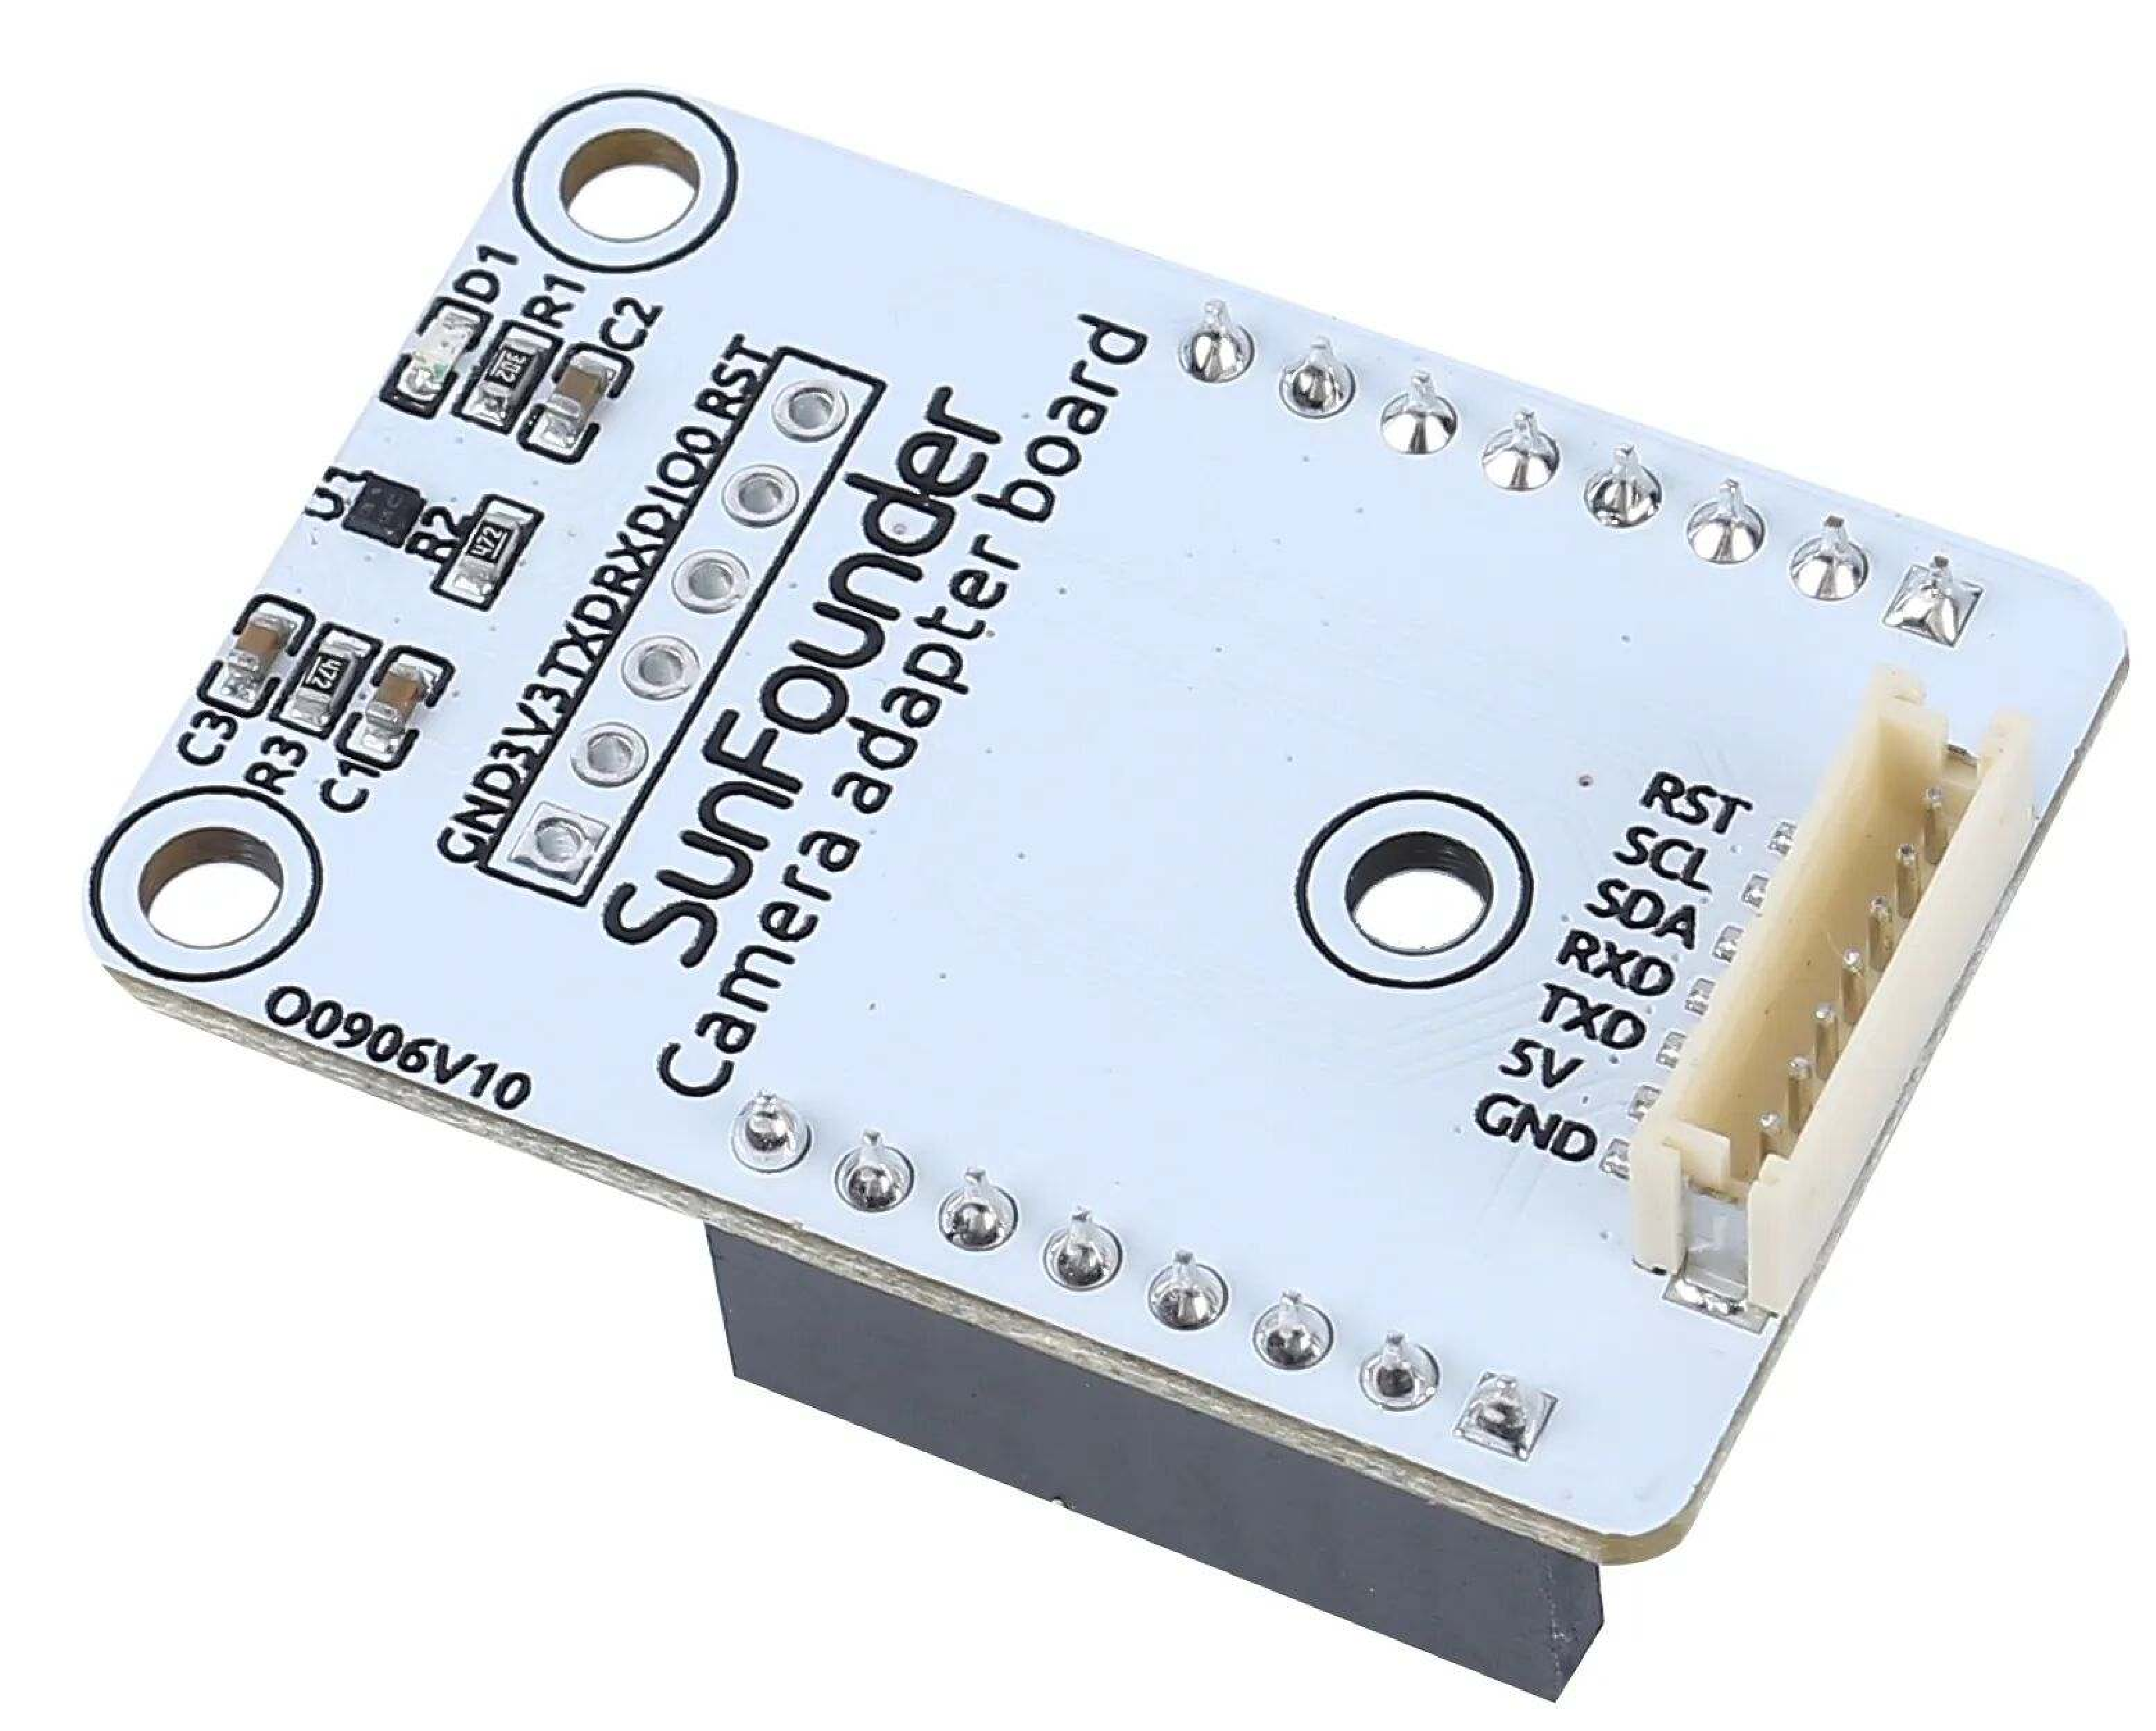
\includegraphics[width=0.8\textwidth]{images/cam_adapter_board.pdf}
\floatnotes{}
%\label{fig:}
\caption{Kamera-Adapterplatine}
\end{figure}

\begin{figure}
\centering
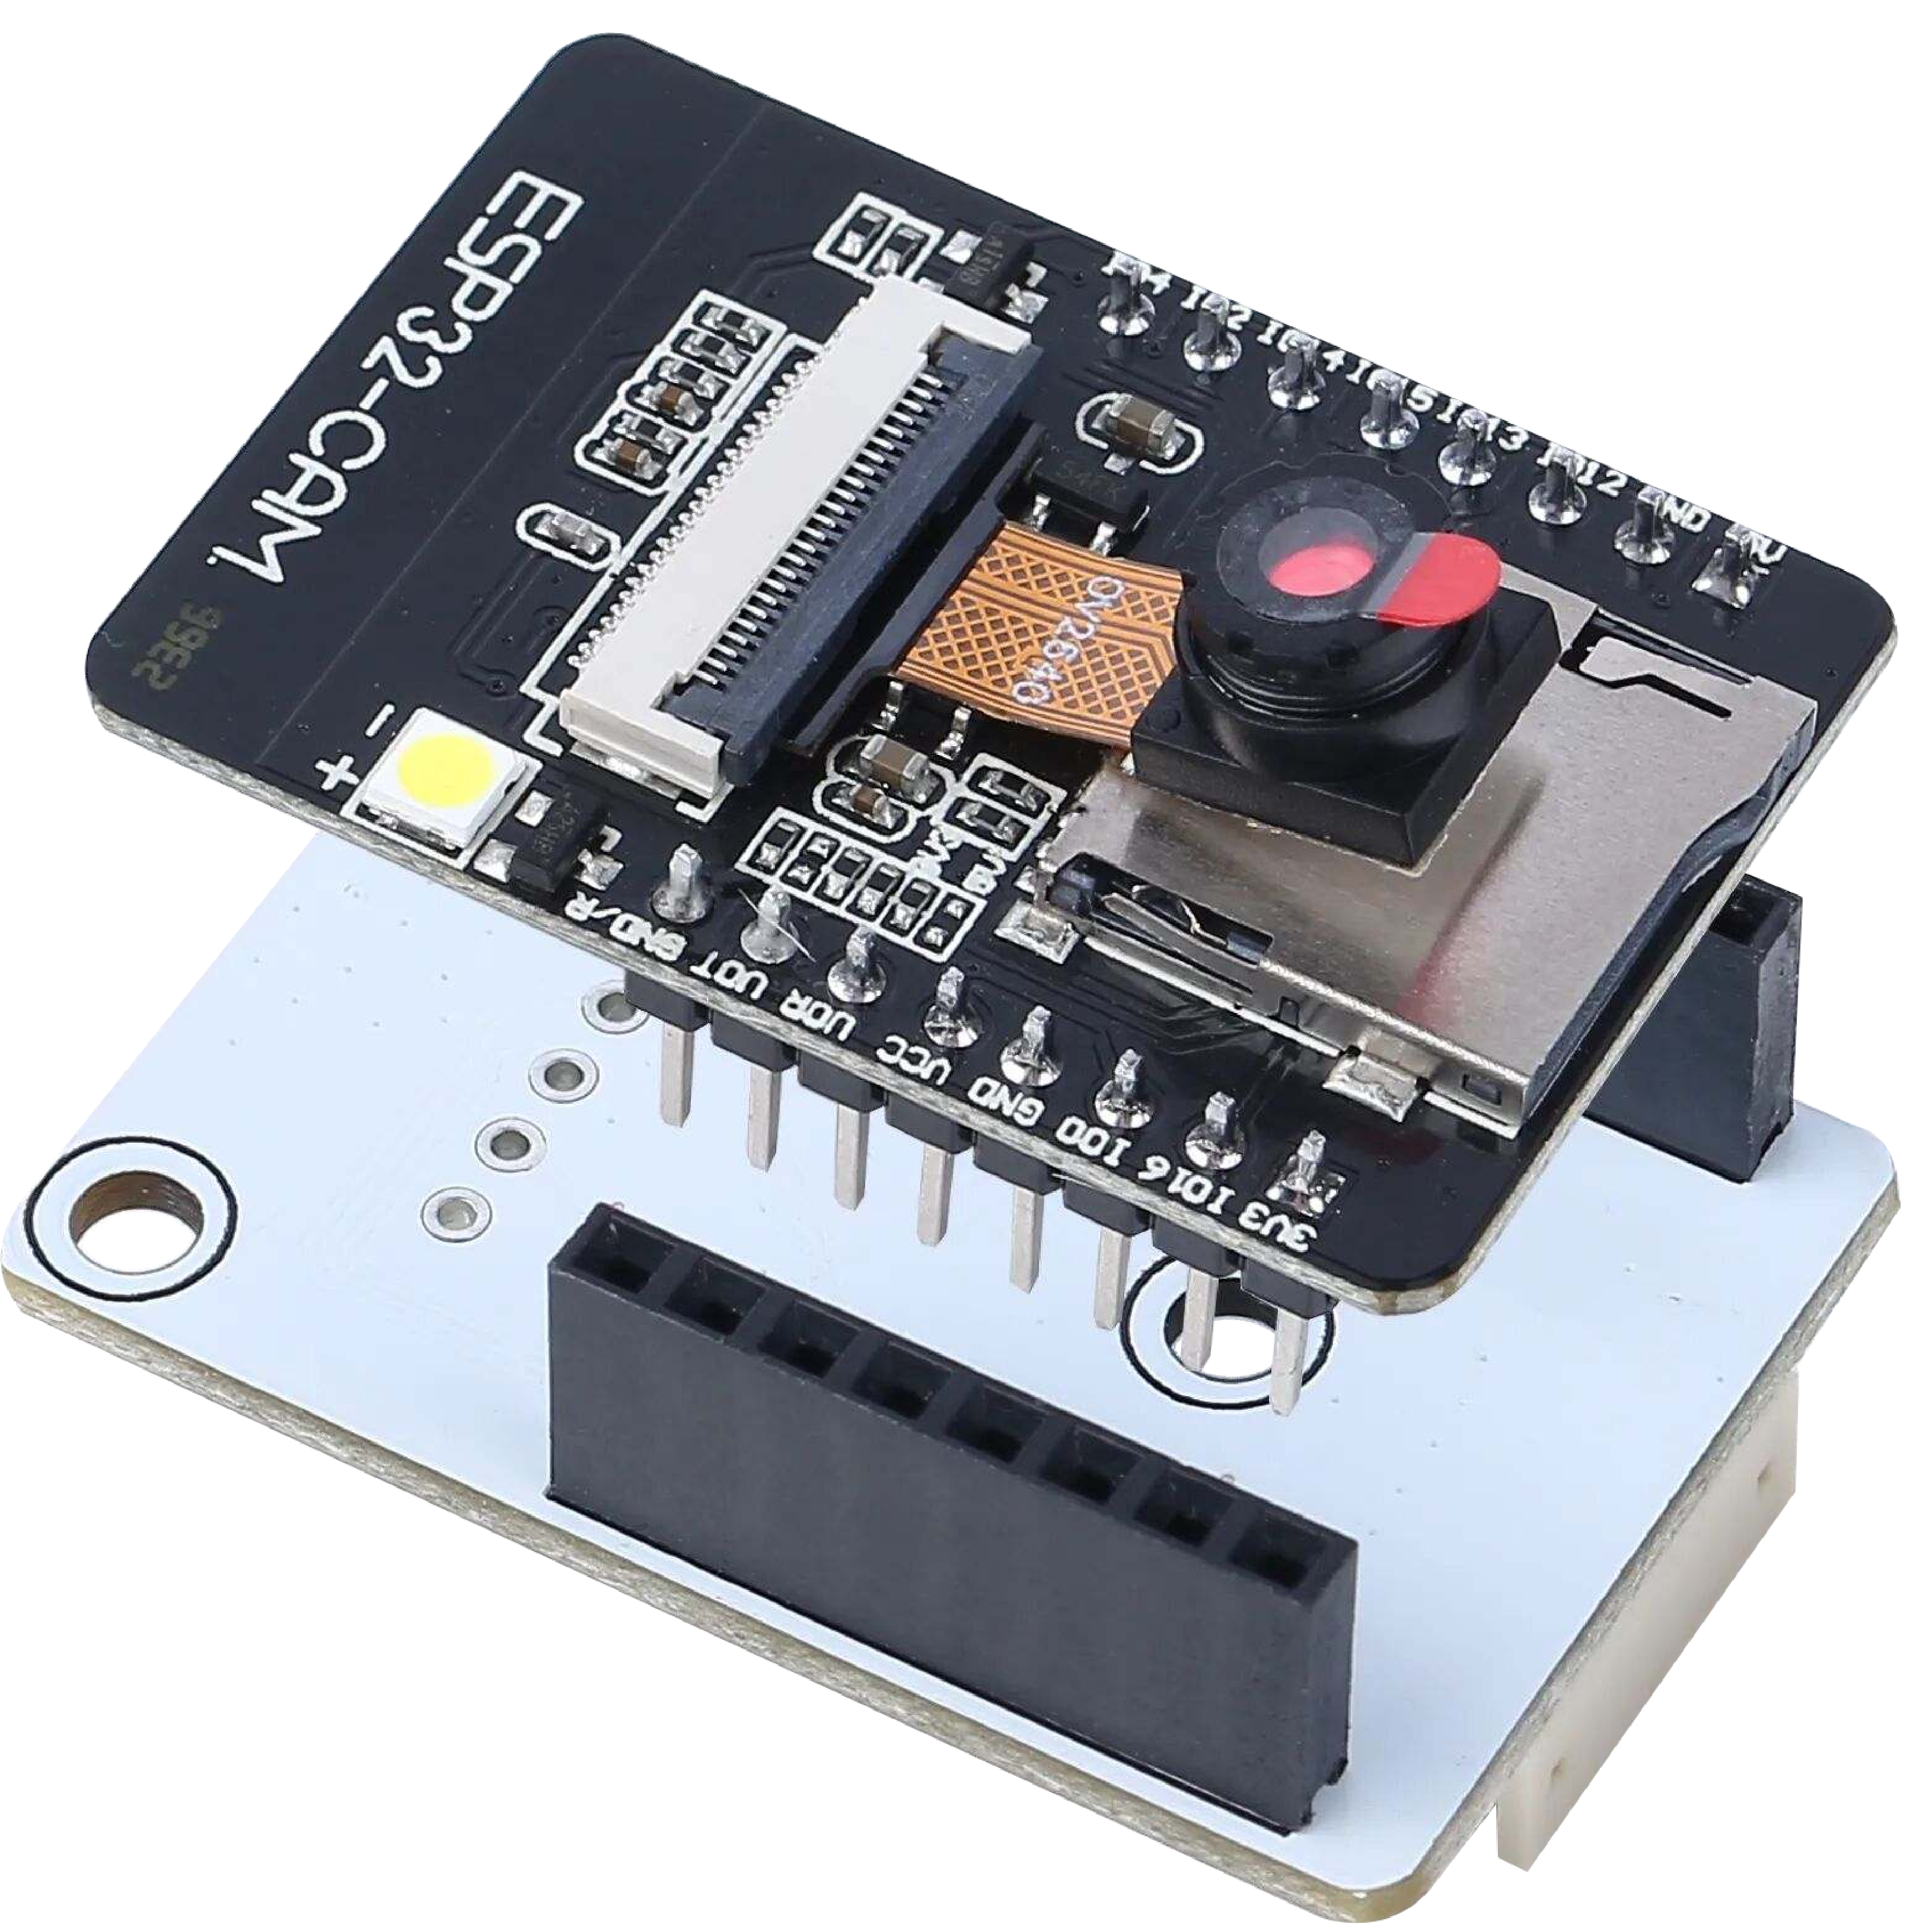
\includegraphics[width=0.8\textwidth]{images/cam_adapter_esp32cam.pdf}
\floatnotes{}
%\label{fig:}
\caption{Kamera-Adapterplatine für ESP32-CAM}
\end{figure}

\begin{figure}
\centering
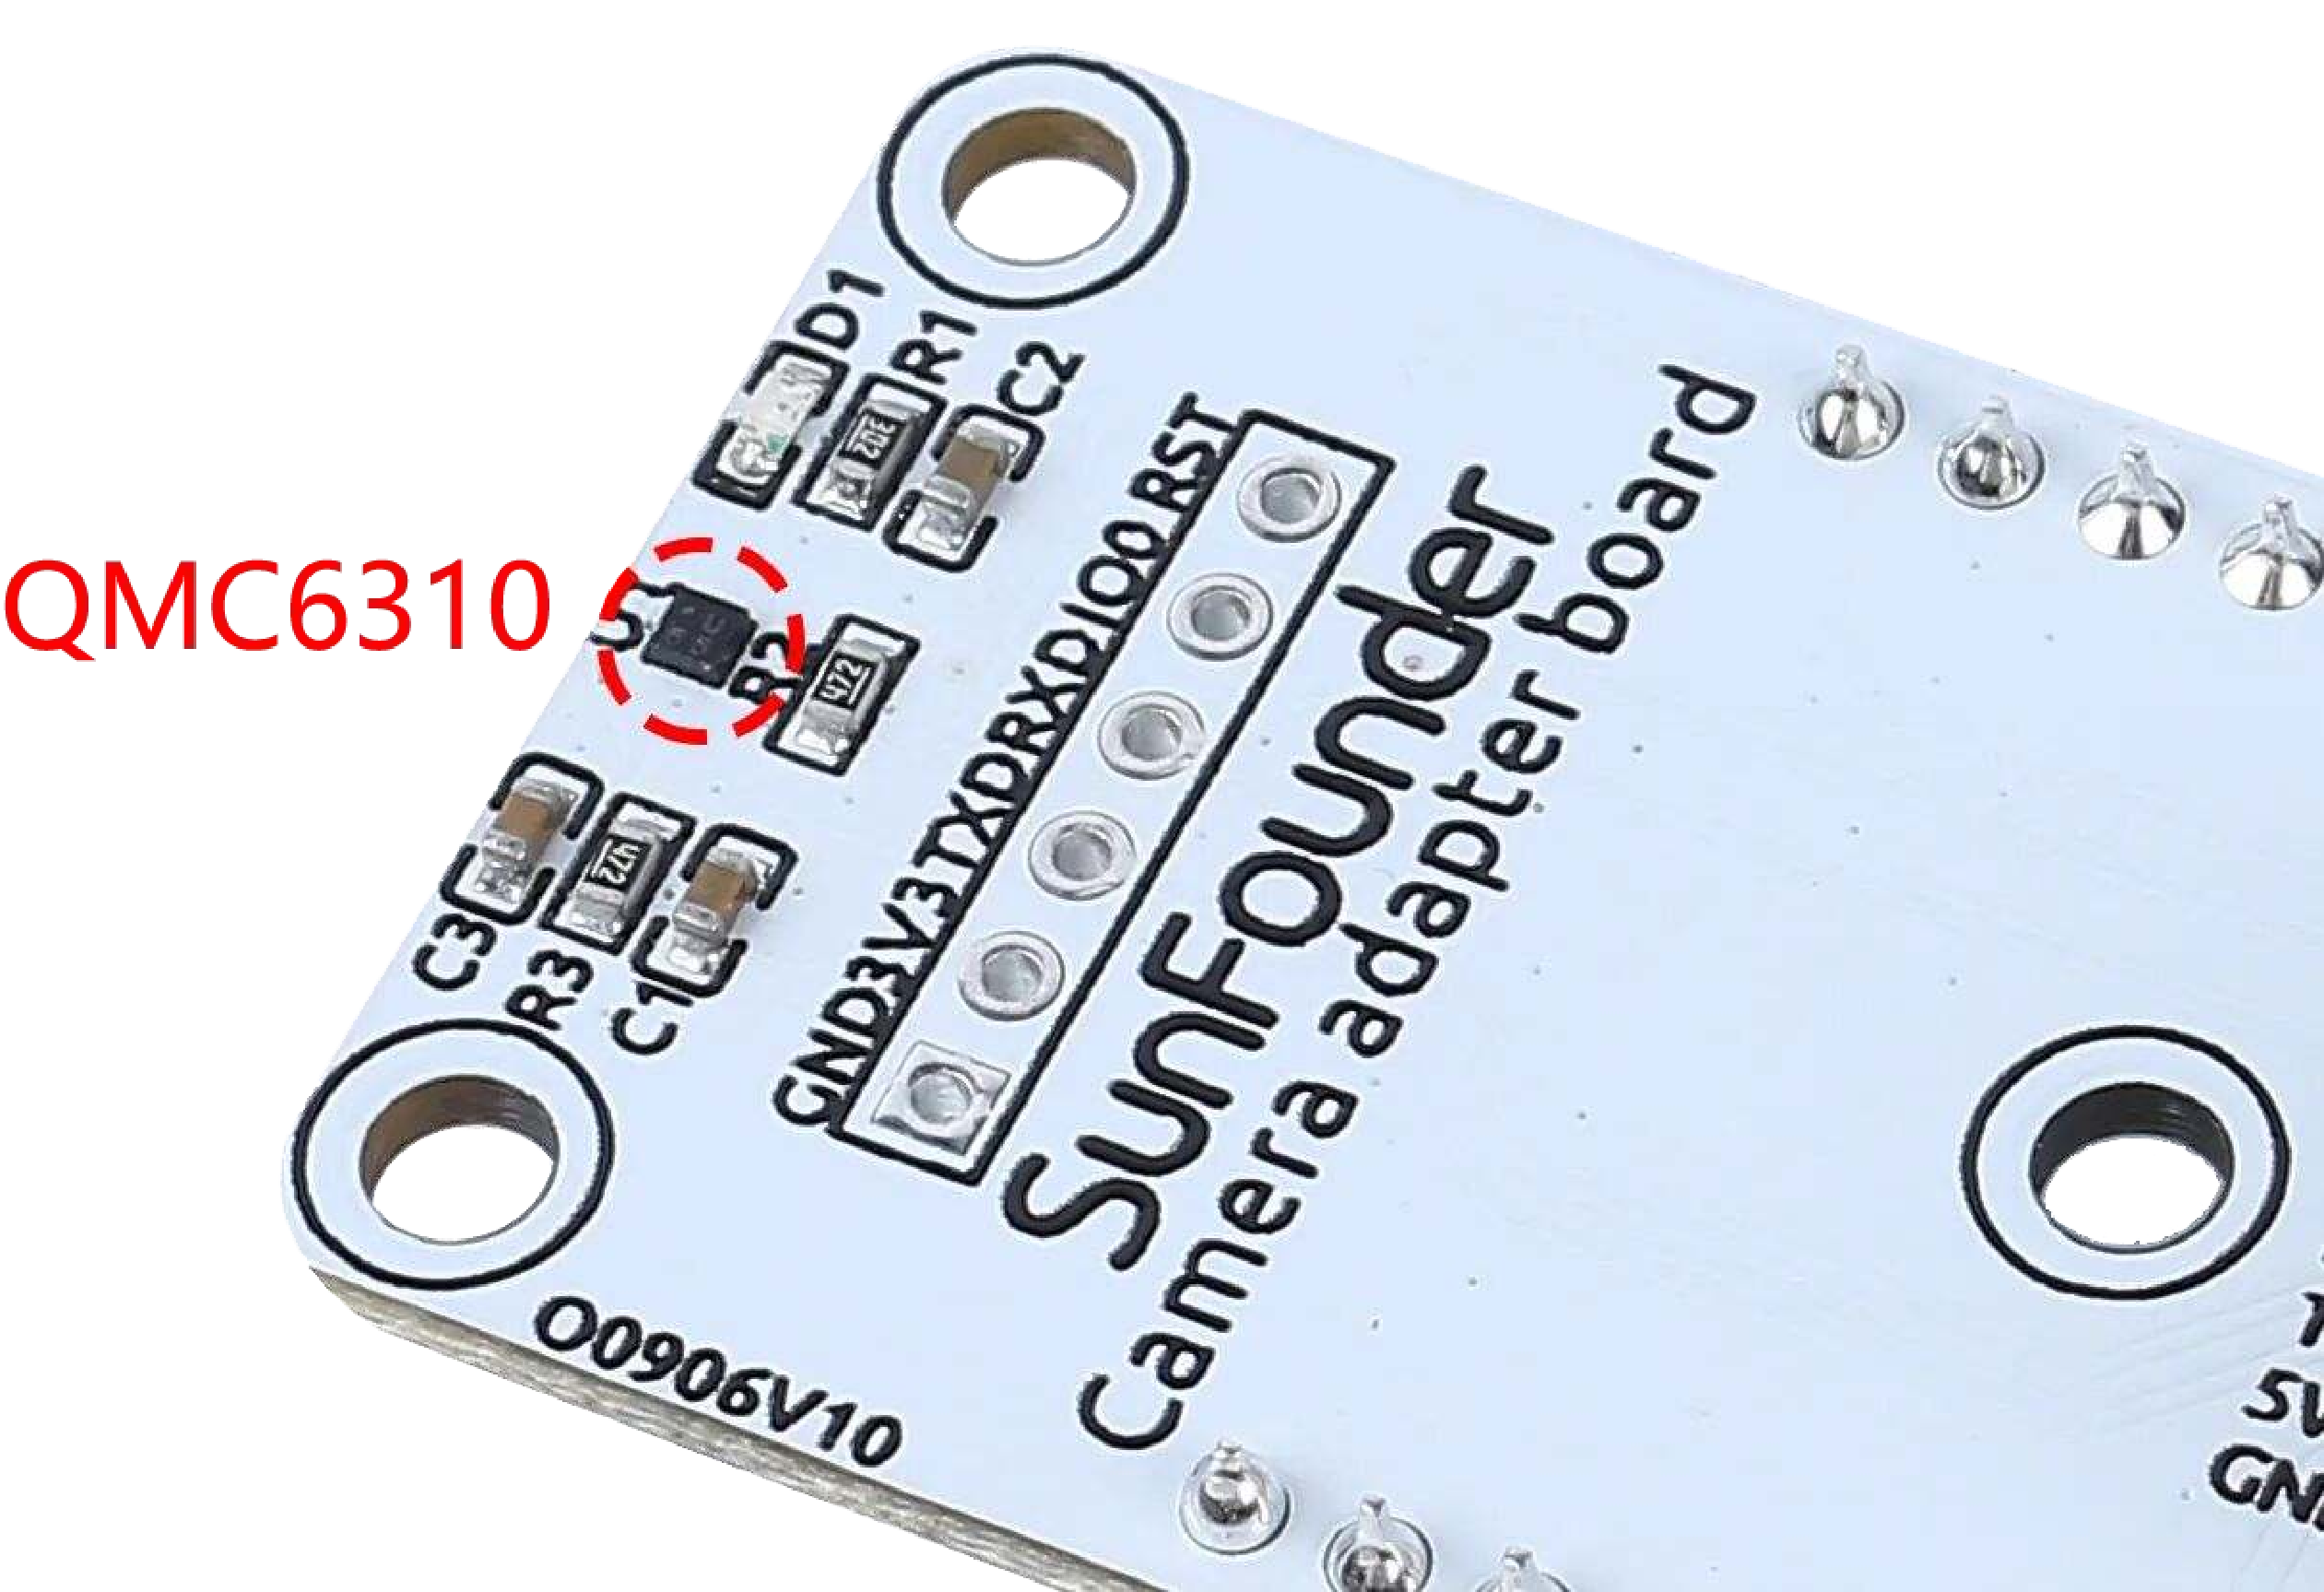
\includegraphics[width=0.8\textwidth]{images/cam_adapter_qmc6310.pdf}
\floatnotes{}
%\label{fig:}
\caption{Dreiaxialer Magnetfeldsensor, Chips QMC6310, geeignet für
Navigation}
\end{figure}

\begin{figure}
\centering
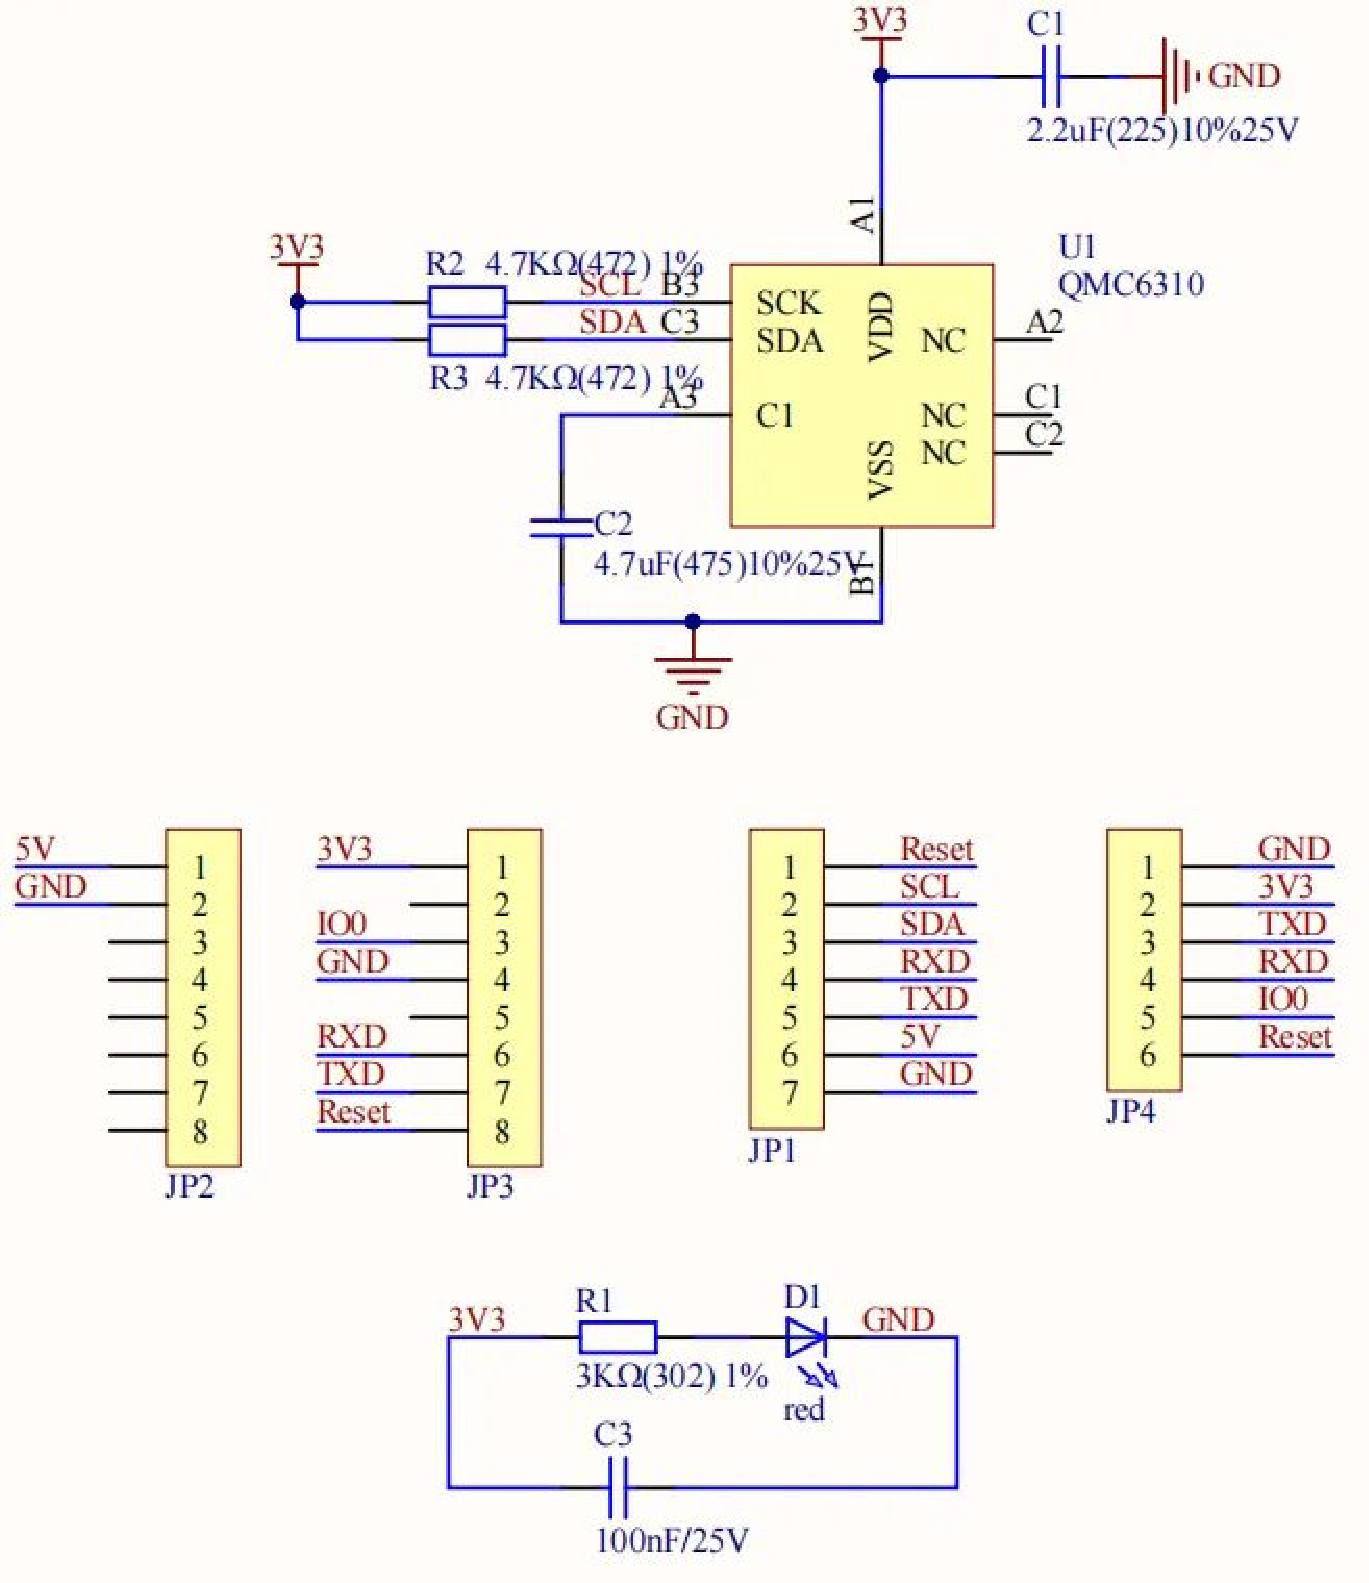
\includegraphics[width=0.8\textwidth]{images/cam_adapter_sche.pdf}
\floatnotes{}
%\label{fig:}
\caption{Kamera-Adapterplatine Schaltplan}
\end{figure}

\begin{itemize}
\item
  \textbf{RST:} Wird verwendet, um die ESP32-CAM zurückzusetzen.
\item
  \textbf{SCL:} Serieller Datenpin für QMC6310
\item
  \textbf{SDA:} Serieller Uhrenpin des QMC6310
\item
  \textbf{RXD:} RXD der ESP32-CAM, Sie benötigen diese beiden seriellen
  Pins, RXD und TXD, um Code auf die ESP32-CAM hochzuladen.
\item
  \textbf{TXD:} TXD der ESP32-CAM
\item
  \textbf{5V:} 5V DC-Eingang
\item
  \textbf{GND:} Masse-Eingang
\item
  \textbf{Kamera-Adapterplatine für ESP32-CAM}:

  \begin{itemize}
  
  \item
    Entwickelt, um die ESP32-CAM zu erweitern und eine einfache Montage
    am Roboter sowie Verkabelung zu ermöglichen.
  \item
    Beinhaltet Anschlüsse wie RST (Reset), SCL und SDA (für QMC6310),
    RXD und TXD (für Code-Upload), 5V DC-Eingang und GND (Masse).
  \end{itemize}
\item
  \textbf{Integration des geomagnetischen Chips QMC6310}:

  \begin{itemize}
  
  \item
    Um Störungen durch Motoren zu vermeiden, ist der QMC6310 auf der
    Adapterplatine platziert, entfernt von Motoren.
  \item
    QMC6310: Dreiaxialer Magnetfeldsensor, geeignet für Anwendungen wie
    E-Kompass, Kartenrotation, Gaming und persönliche Navigation.
  \end{itemize}
\item
  \textbf{Technische Details der Kamera-Adapterplatine}:

  \begin{itemize}
  
  \item
    Betriebsspannung: 5V.
  \item
    Schnittstellenmodell: ZH1.5, 7P.
  \item
    Abmessungen: 40mm x 27mm x 15mm.
  \item
    Kommunikationsprotokoll: UART und I2C.
  \end{itemize}
\item
  \textbf{Eigenschaften des QMC6310}:

  \begin{itemize}
  
  \item
    Integriert magnetische Sensoren und Signalzustands-ASIC auf einem
    Siliziumchip.
  \item
    Nutzt hochauflösende, magnetoresistive Technologie mit einem
    16-Bit-ADC-ASIC.
  \item
    Bietet Vorteile wie geringes Rauschen, hohe Genauigkeit, geringer
    Stromverbrauch, Offset- und Temperaturkompensation.
  \item
    Kompassgenauigkeit von 1° bis 2°.
  \item
    Einfache Schnittstellenanbindung über I2C-Serienbus.
  \item
    Verpackt in einem 1,2x1,2x0,53mm\^{}3 großen, 8-Pin-LGA-Gehäuse.
  \end{itemize}
\end{itemize}

\hypertarget{ultraschallmodul}{%
\subsection{Ultraschallmodul}\label{ultraschallmodul}}

\begin{figure}
\centering
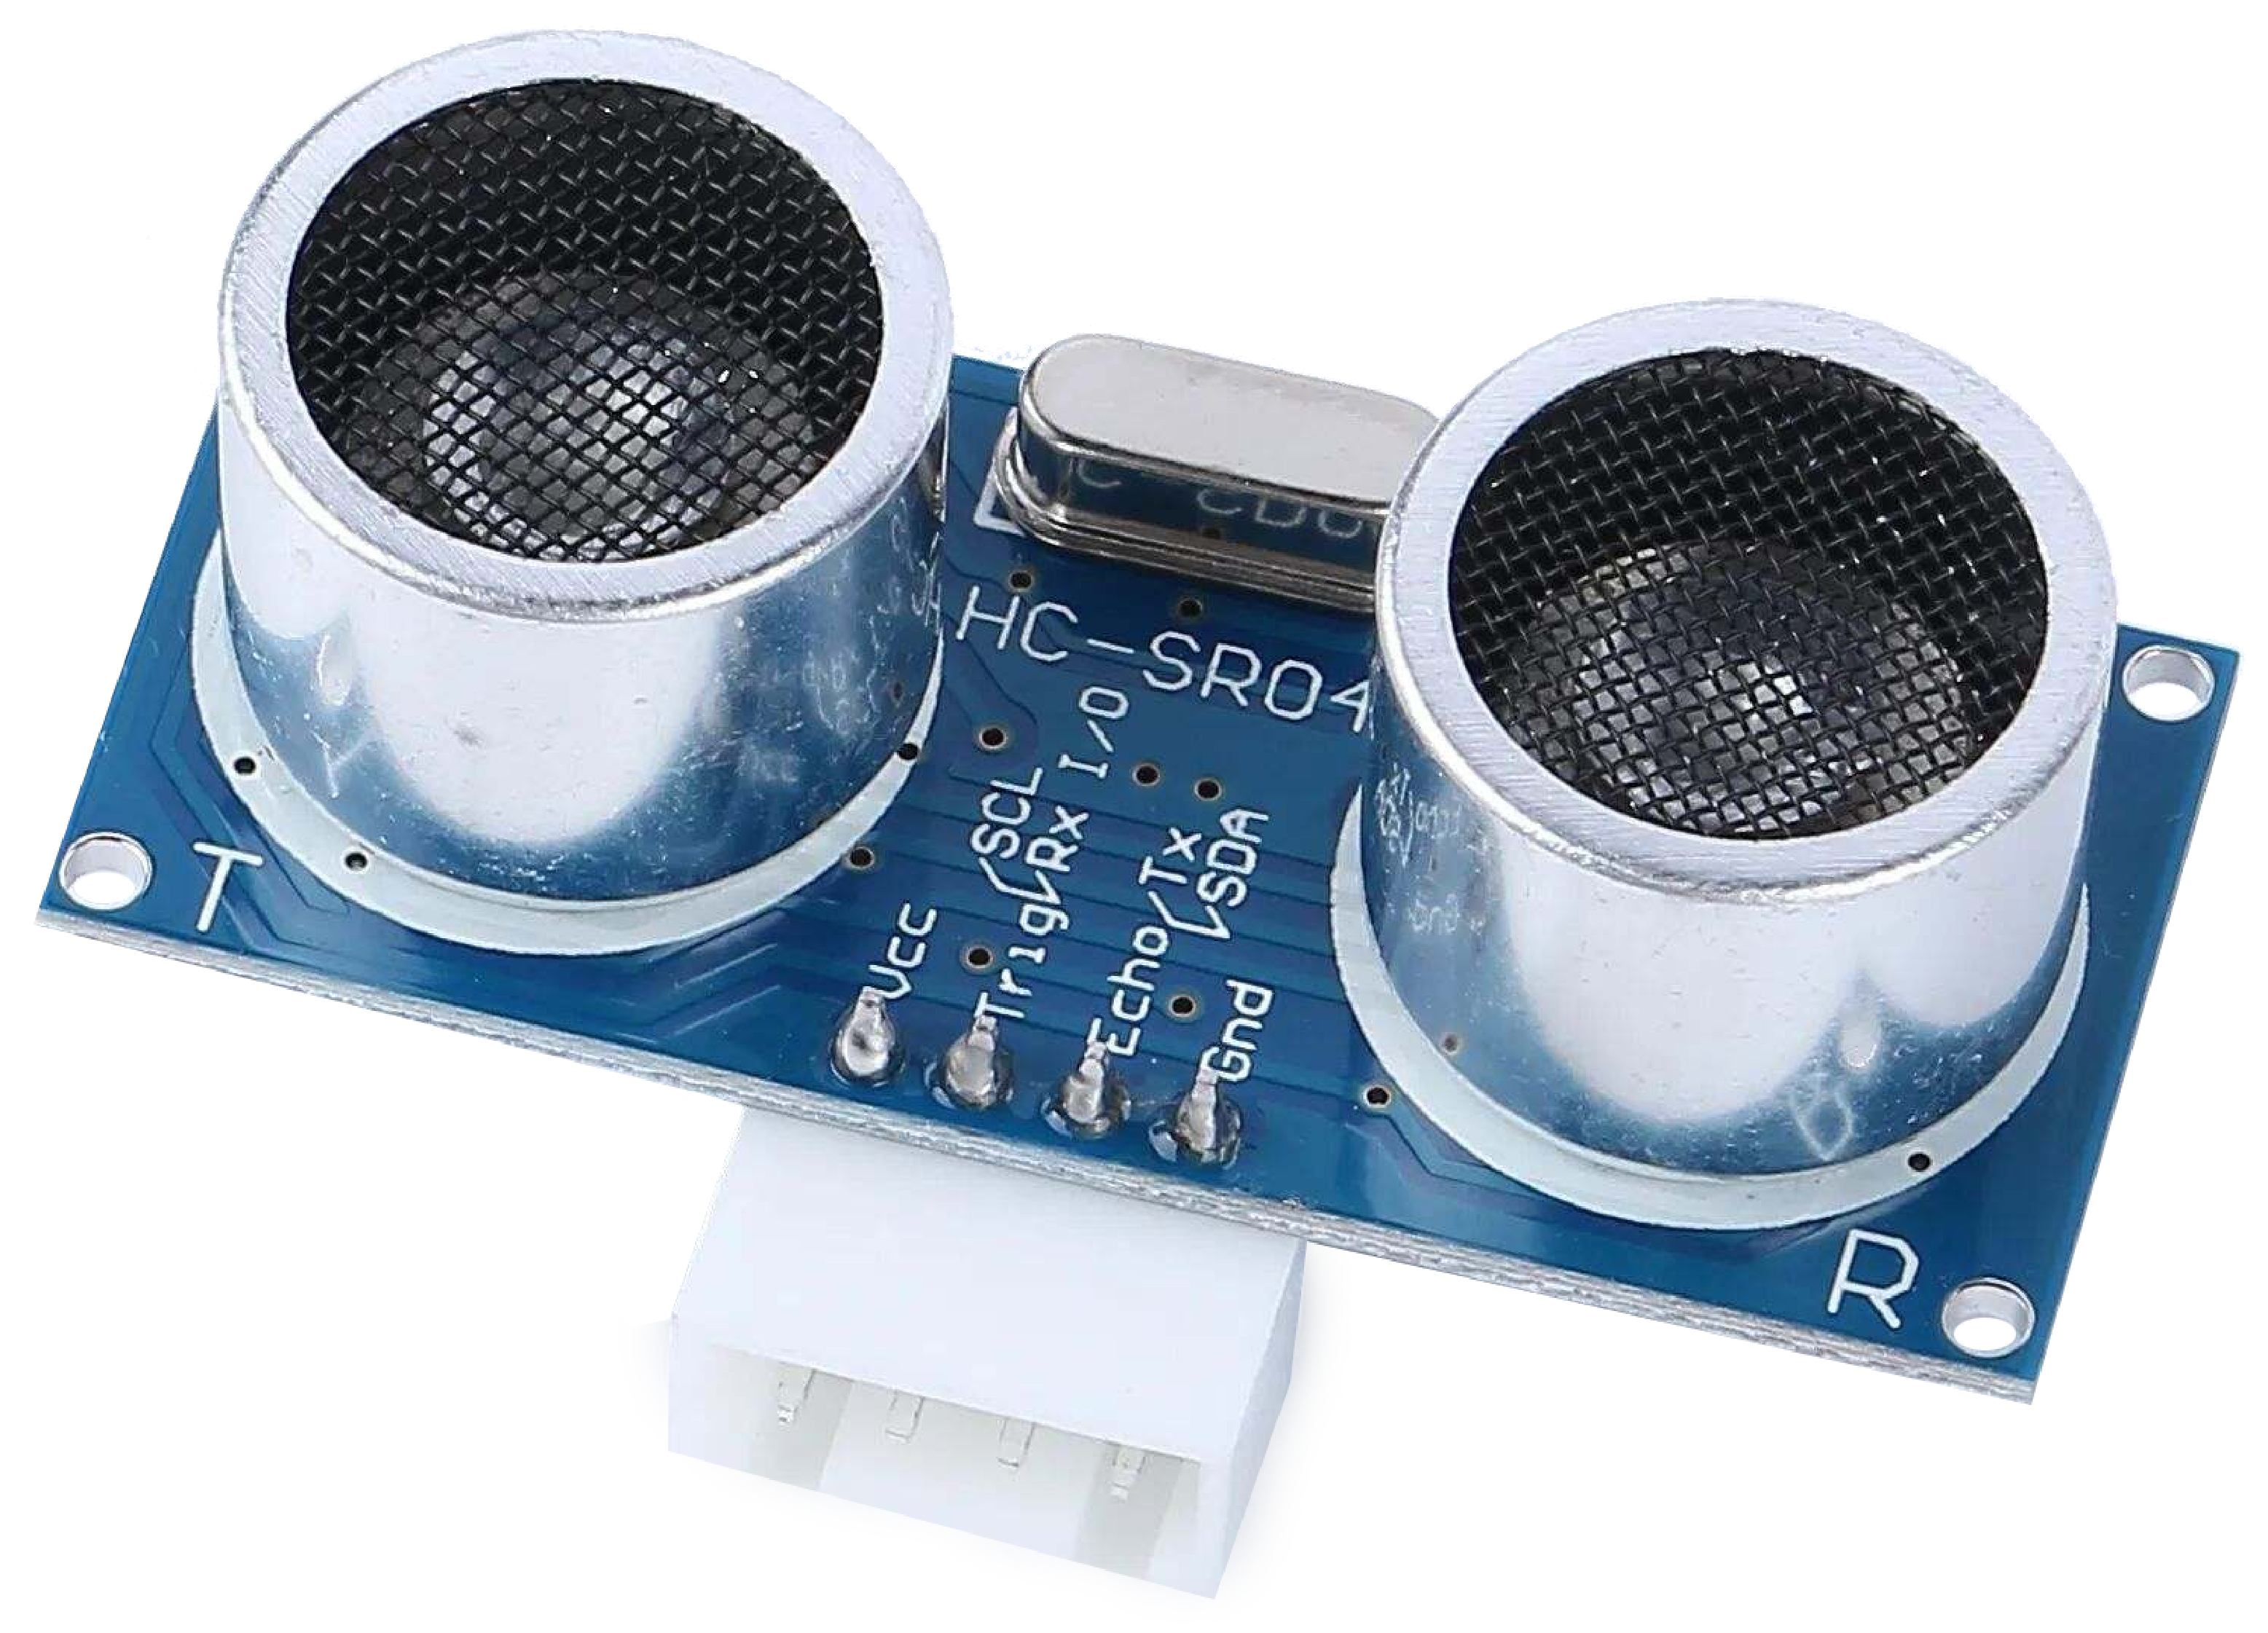
\includegraphics[width=0.8\textwidth]{images/ultrasonic_pic.pdf}
\floatnotes{}
%\label{fig:}
\caption{Ultraschallmodul}
\end{figure}

\begin{itemize}

\item
  \textbf{HC-SR04 Ultraschall-Abstandssensor}:

  \begin{itemize}
  
  \item
    Bietet berührungslose Messungen im Bereich von 2 cm bis 400 cm.
  \item
    Bereichsgenauigkeit: bis zu 3 mm.
  \item
    Enthält Ultraschall-Sender, Empfänger und Steuerschaltung.
  \end{itemize}
\item
  \textbf{Anschluss}:

  \begin{itemize}
  
  \item
    Vier Pins: VCC (5V Versorgung), TRIG (Trigger-Pulseingang), ECHO
    (Echo-Pulseausgang), GND (Erdung).
  \end{itemize}
\item
  \textbf{Merkmale}:

  \begin{itemize}
  
  \item
    Betriebsspannung: DC5V.
  \item
    Betriebsstrom: 16mA.
  \item
    Arbeitsfrequenz: 40Hz.
  \item
    Maximaler Messbereich: 500cm.
  \item
    Minimaler Messbereich: 2cm.
  \item
    Trigger-Eingangssignal: 10uS TTL-Impuls.
  \item
    Echo-Ausgangssignal: TTL-Pegelsignal, Dauer proportional zur
    Entfernung.
  \item
    Steckverbinder: XH2.54-4P.
  \item
    Abmessungen: 46x20.5x15 mm.
  \end{itemize}
\item
  \textbf{Funktionsprinzip}:

  \begin{itemize}
  
  \item
    Auslösen eines 10us hohen Signals über IO-Trigger.
  \item
    Senden eines 8-Zyklus-Bursts von Ultraschall bei 40 kHz und
    Empfangen des Echo-Signals.
  \item
    \textbf{Messprinzip} Sensor misst Entfernungen durch das Senden und
    Empfangen von Ultraschallwellen. Der Prozess beginnt mit einem
    Trigger-Signal und endet mit der Berechnung der Distanz basierend
    auf der Echo-Zeit.
  \end{itemize}
\item
  \textbf{Anwendungshinweise}:

  \begin{itemize}
  
  \item
    Modul nicht unter Strom anschließen; zuerst GND verbinden.
  \item
    Das Messobjekt sollte mindestens 0,5 Quadratmeter groß und möglichst
    flach sein für präzise Ergebnisse.
  \end{itemize}
\end{itemize}

\hypertarget{ir-hindernisvermeidungsmodul}{%
\subsection{IR-Hindernisvermeidungsmodul}\label{ir-hindernisvermeidungsmodul}}

\begin{figure}
\centering
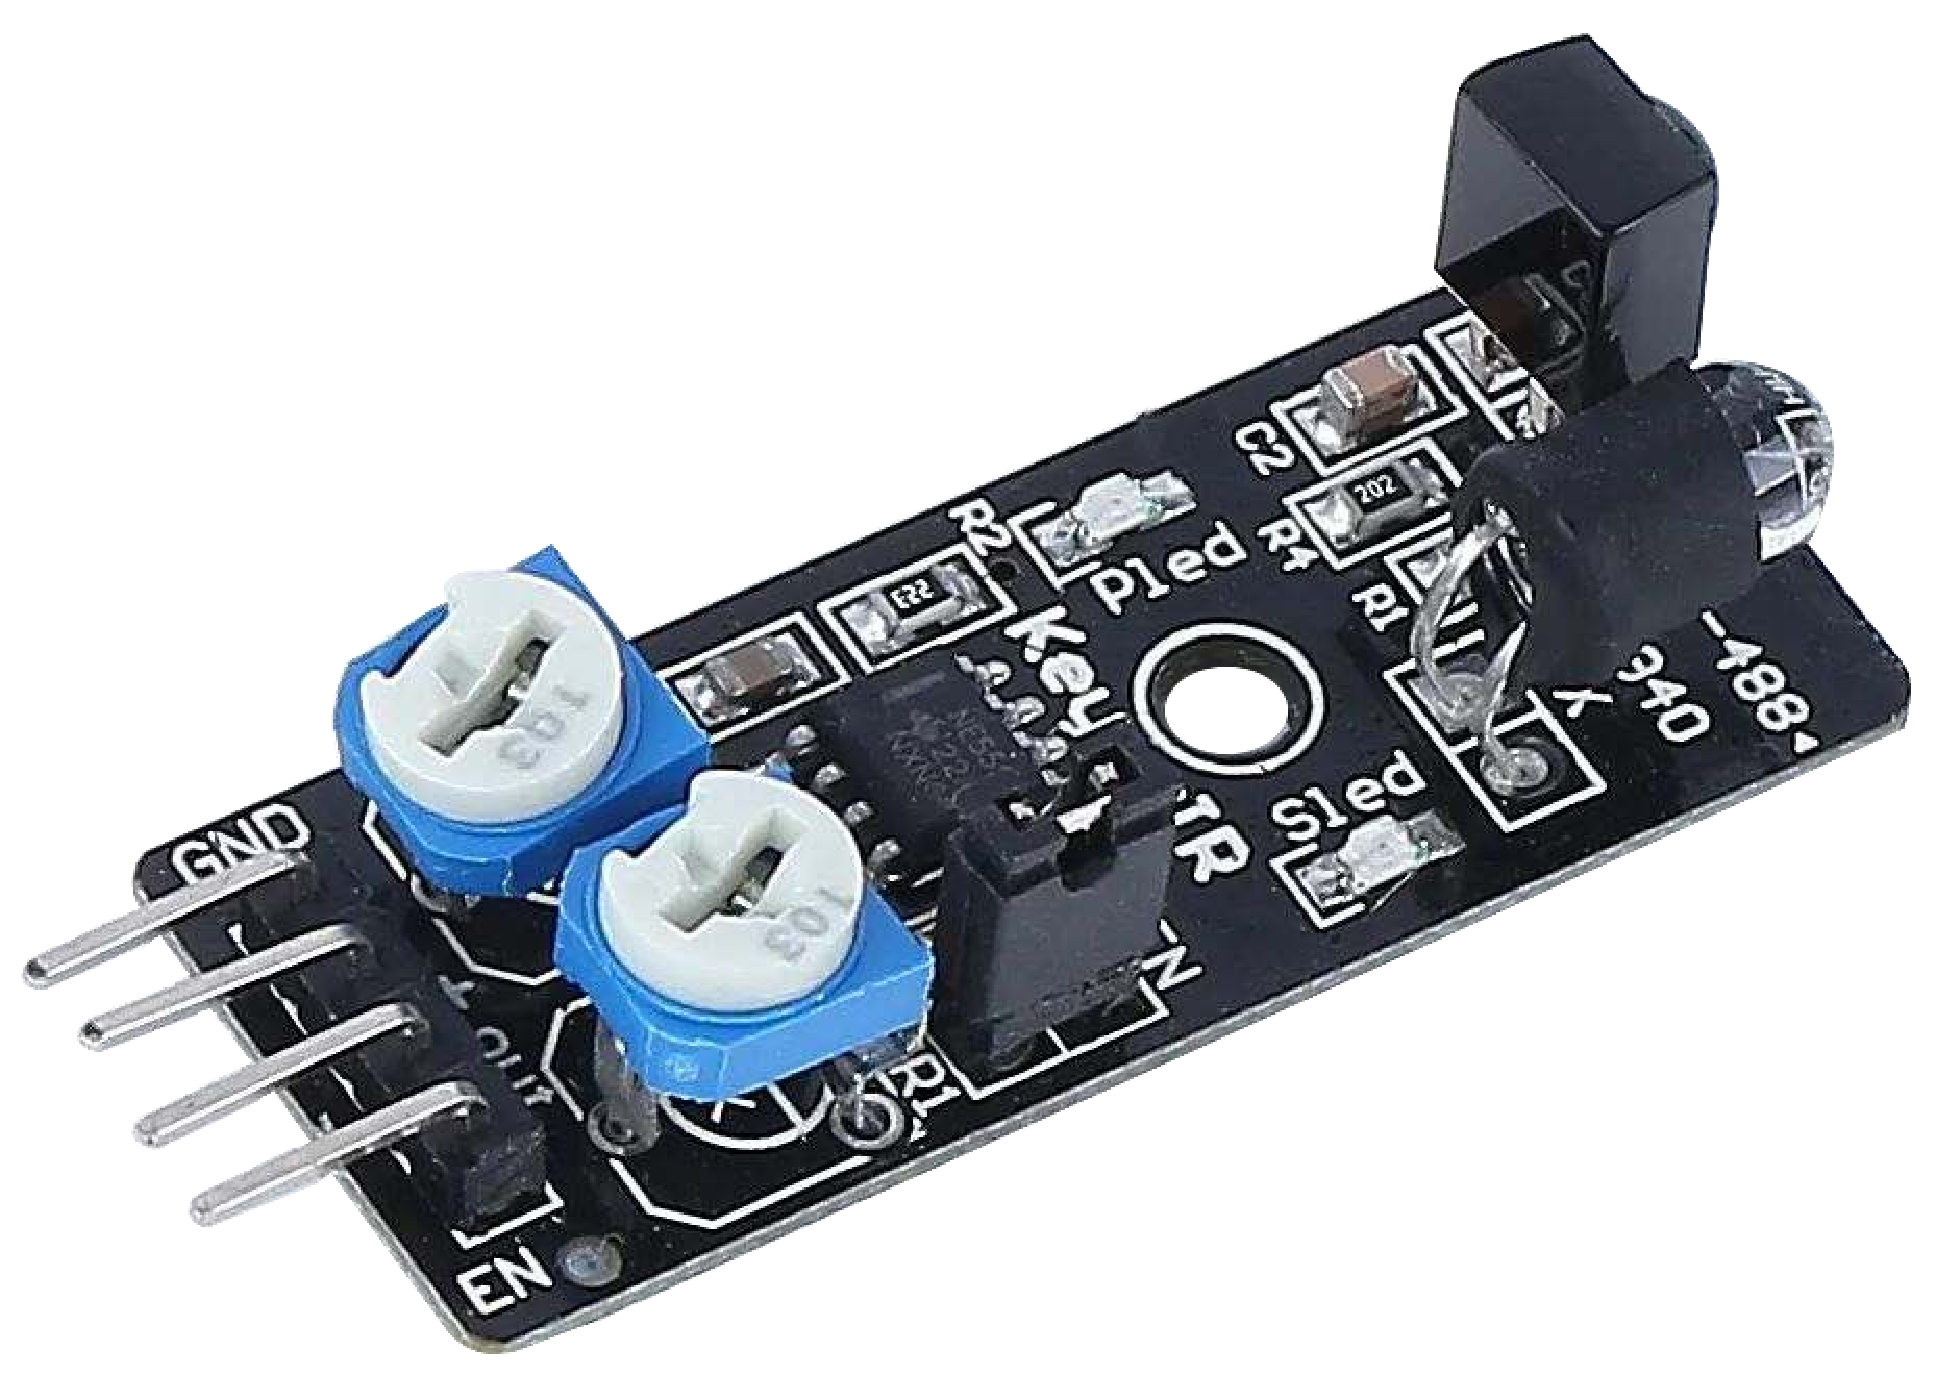
\includegraphics[width=0.8\textwidth]{images/ir_avoid.pdf}
\floatnotes{}
%\label{fig:}
\caption{IR Hindernisvermeidungsmodul}
\end{figure}

\begin{figure}
\centering
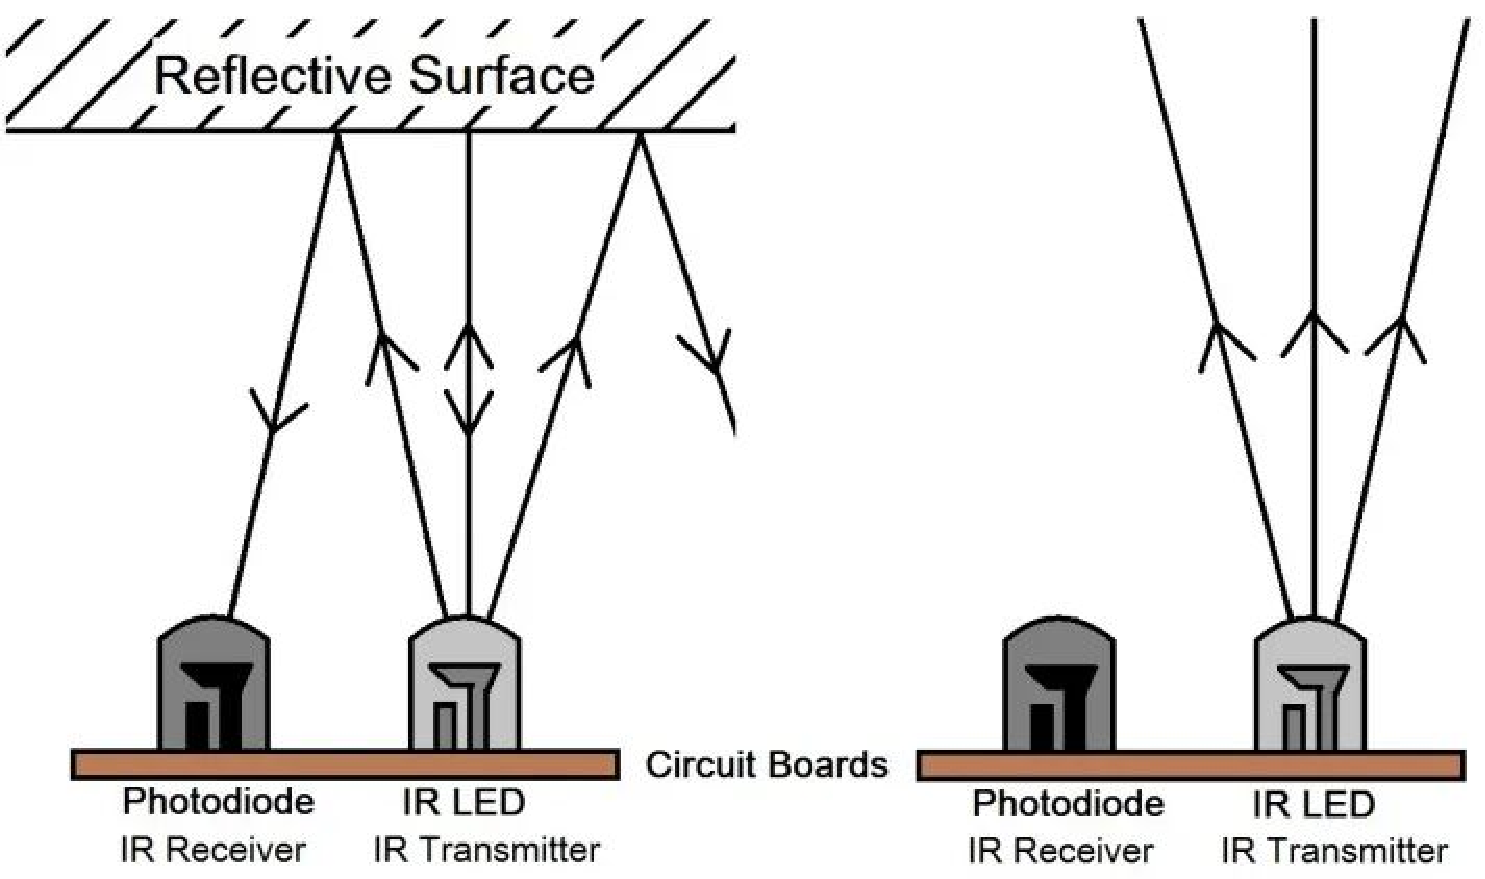
\includegraphics[width=0.8\textwidth]{images/ir_receive.pdf}
\floatnotes{}
%\label{fig:}
\caption{IR Empfängermodul}
\end{figure}

\begin{itemize}

\item
  \textbf{IR-Hindernisvermeidungsmodul}:

  \begin{itemize}
  
  \item
    Dient der Erkennung von Objekten im Bereich von 2 cm bis 40 cm.
  \item
    Die Reflexionsniveaus variieren je nach Farbe des Objekts, wobei
    dunklere Objekte den Erfassungsbereich verkürzen.
  \end{itemize}
\item
  \textbf{Pin-Definitionen}:

  \begin{itemize}
  
  \item
    GND: Erdung.
  \item
    +: Stromversorgung, zwischen 3,3 und 5V DC.
  \item
    Out: Standardmäßig hoch; wird niedrig bei Hinderniserkennung.
  \item
    EN: Enable-Pin, standardmäßig mit GND verbunden, hält das Modul
    aktiv.
  \end{itemize}
\item
  \textbf{Funktionsweise}:

  \begin{itemize}
  
  \item
    Beinhaltet ein IR-Sender-Empfänger-Paar.
  \item
    Der Sender emittiert Infrarotlicht, das von Hindernissen reflektiert
    und vom Empfänger detektiert wird, woraufhin ein niedriges Signal
    ausgegeben wird.
  \end{itemize}
\item
  \textbf{EN-Pin und Jumper}:

  \begin{itemize}
  
  \item
    Der niedrige Zustand des EN-Pins aktiviert das Modul.
  \item
    Der Jumper verbindet den EN-Pin mit GND; für programmierte Steuerung
    wird sie entfernt.
  \end{itemize}
\item
  \textbf{Potentiometer für Einstellungen}:

  \begin{itemize}
  
  \item
    Zwei Potentiometer zur Einstellung der Sendeleistung und -frequenz.
  \item
    Ermöglicht Anpassung der effektiven Entfernung.
  \end{itemize}
\item
  \textbf{Kalibrierung}:

  \begin{itemize}
  
  \item
    Erfordert präzise Ausrichtung und Anpassung der Potentiometer, um
    die gewünschte Erfassungsdistanz zu erreichen.
  \end{itemize}
\item
  \textbf{Technische Spezifikationen}:

  \begin{itemize}
  
  \item
    Betriebsspannung: 3,3 V bis 5 V.
  \item
    Ausgang: Digital (Ein/Aus).
  \item
    Einstellschwelle: Durch 2 Potentiometer einstellbar.
  \item
    Distanzbereich: 2 bis 40 cm.
  \item
    Betriebstemperatur: -10 °C bis +50 °C.
  \item
    Effektiver Winkel: 35°.
  \item
    I/O-Schnittstelle: 4-Draht (- / + / S / EN).
  \item
    Abmessungen: 45 x 16 x 10 mm.
  \item
    Gewicht: 9 g.
  \end{itemize}
\end{itemize}

\hypertarget{rgb-led-streifen}{%
\subsection{RGB-LED-Streifen}\label{rgb-led-streifen}}

\begin{figure}
\centering
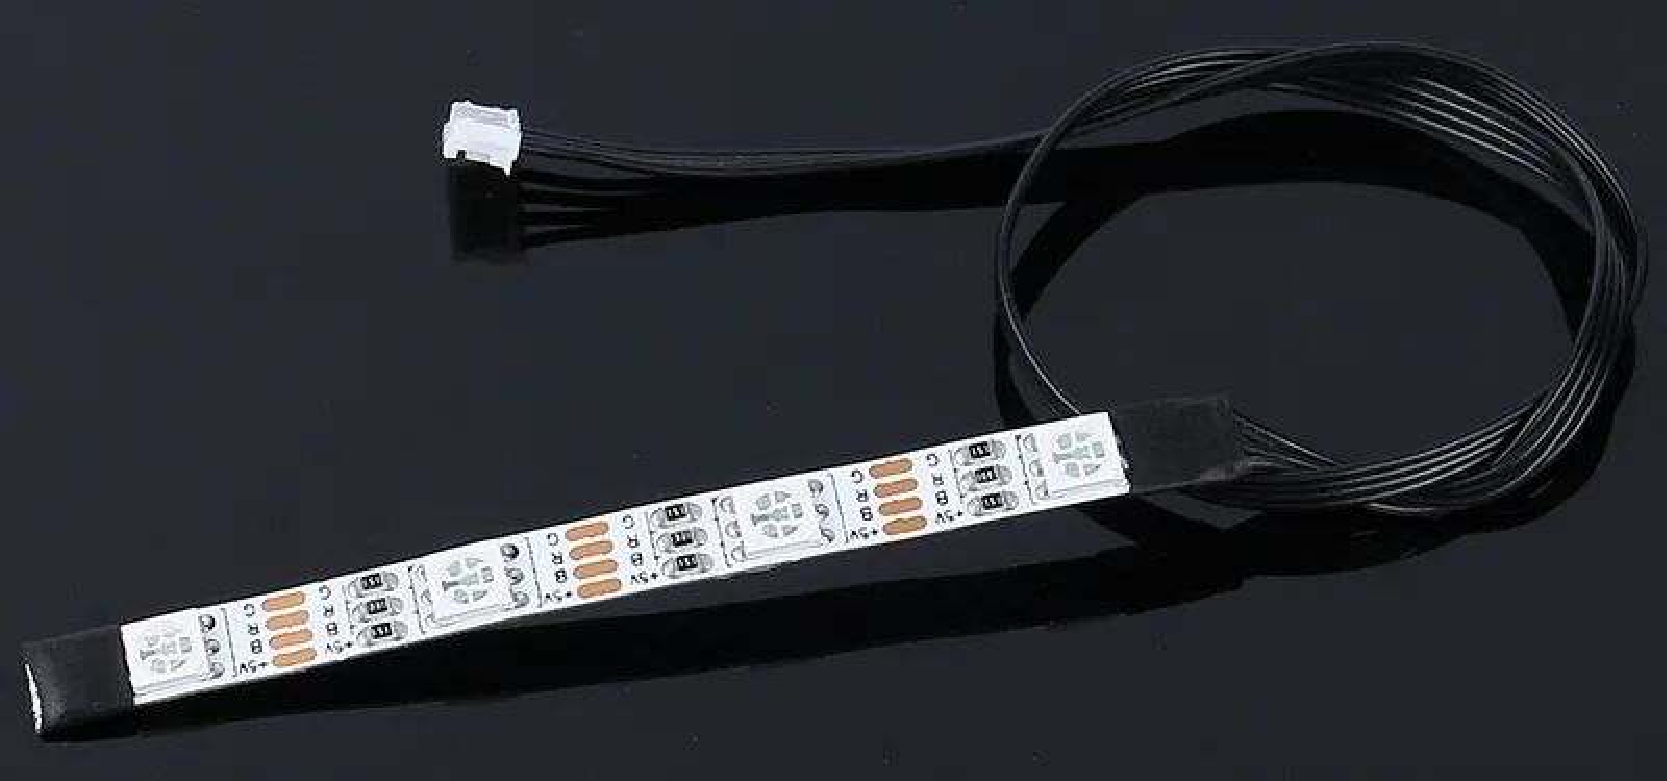
\includegraphics[width=0.8\textwidth]{images/4_rgb_strip.pdf}
\floatnotes{}
%\label{fig:}
\caption{4-Pin RGB-LED-Streifen}
\end{figure}

\begin{figure}
\centering
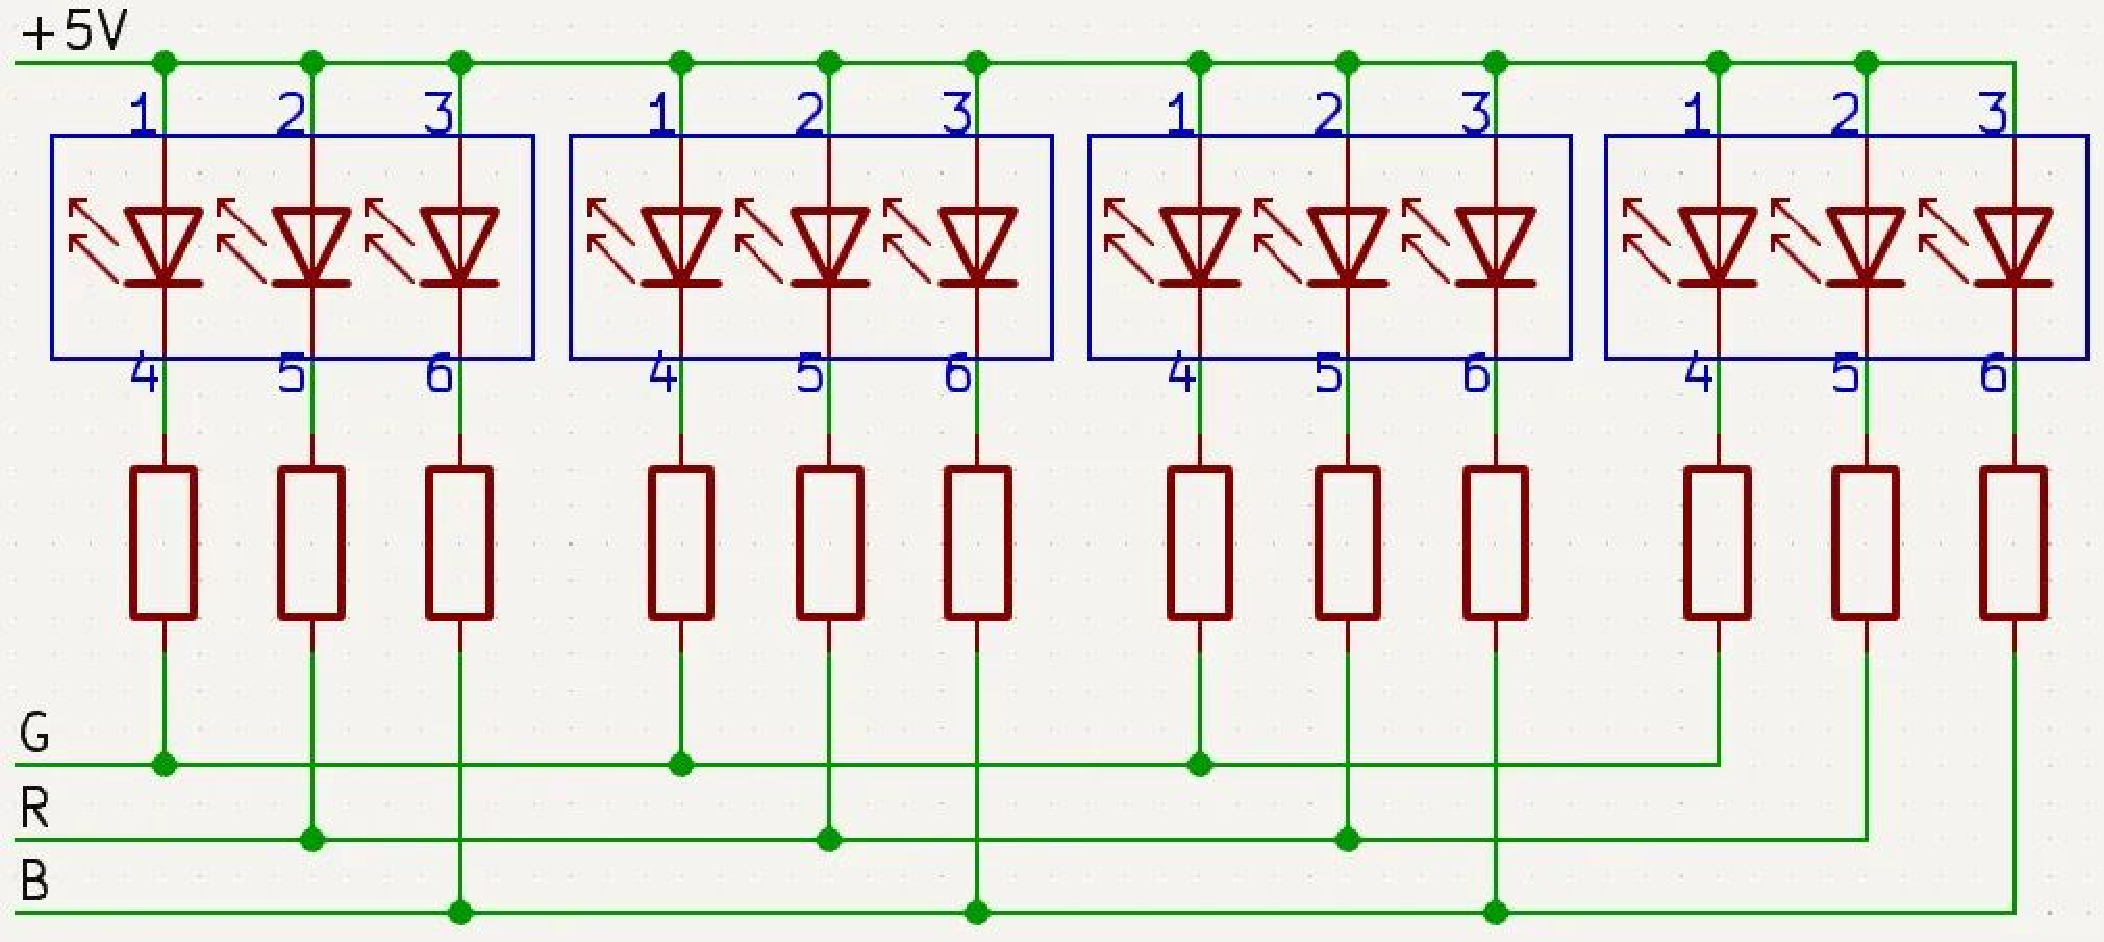
\includegraphics[width=0.8\textwidth]{images/rgb_strip_sche.pdf}
\floatnotes{}
%\label{fig:}
\caption{RGB-LED-Streifen Schaltplan}
\end{figure}

\hypertarget{eigenschaften-von-rgb-led-streifen}{%
\subsubsection{Eigenschaften von
RGB-LED-Streifen}\label{eigenschaften-von-rgb-led-streifen}}

\begin{itemize}

\item
  Verwendet vier R5050 RGB-LEDs für die Farberzeugung durch Mischung von
  Rot, Blau und Grün.
\item
  Konfiguration mit gemeinsamer Anode (+5V) und individuellen Kathoden
  (B, R, G) für jede Farb-LED.
\item
  Jede LED funktioniert unabhängig, erlaubt das Schneiden des Streifens
  an markierten Stellen ohne Beeinträchtigung anderer Segmente.
\item
  Flexibel und einfach zu installieren dank FPC-Platine mit
  doppelseitigem Klebstoff.
\end{itemize}

\hypertarget{r5050-rgb-led}{%
\subsubsection{R5050 RGB-LED}\label{r5050-rgb-led}}

\begin{itemize}

\item
  Kombiniert rote, blaue und grüne LEDs in einem Gehäuse für breite
  Farbpalette.
\item
  Individuelle Steuerung jeder LED-Farbe durch separate Pins.
\item
  Ermöglicht anpassbare Farbbeleuchtung für dekorative Beleuchtung und
  Displaytechnologien.
\end{itemize}

\hypertarget{technische-merkmale}{%
\subsubsection{Technische Merkmale}\label{technische-merkmale}}

\begin{itemize}

\item
  Arbeitsspannung: DC5V.
\item
  Vollfarbe RGB.
\item
  Arbeitstemperatur: -15 °C bis 50 °C.
\item
  RGB-Typ: 5050RGB.
\item
  Strom: 150mA pro Einzelschaltkreis.
\item
  Leistung: 1.5W.
\item
  Dicke des Lichtstreifens: 2mm; Breite: 5.5mm.
\item
  Anschlusskabel: ZH1.5-4P, 25cm Länge, 28AWG, in Schwarz.
\end{itemize}

\hypertarget{anwendung-und-konfiguration}{%
\subsubsection{Anwendung und
Konfiguration}\label{anwendung-und-konfiguration}}

\begin{itemize}

\item
  Mehrere R5050 RGB-LEDs werden auf einem flexiblen Schaltkreis smart
  angeordnet.
\item
  Gemeinsame Anoden aller LEDs sind verbunden, während Kathoden an
  jeweilige Farbleitungen angeschlossen sind.
\item
  Diese Anordnung unterstützt effiziente Farbmischung und
  Lichtintensitätssteuerung.
\end{itemize}

\hypertarget{gesamtstromverbrauch}{%
\subsubsection{Gesamtstromverbrauch}\label{gesamtstromverbrauch}}

Angenommen, der Gesamtstromverbrauch aller drei farbigen LEDs (Rot,
Grün, Blau) in einem 5050 RGB-LED-Paket beträgt 150 mA und jede LED wird
mit einer Spannung von 5V betrieben.

$I_{gesamt} = 4 \times 150\, \text{mA} = 600\, \text{mA}$

\hypertarget{gesamtleistung}{%
\subsubsection{Gesamtleistung}\label{gesamtleistung}}

Die Leistung ($P$) kann mit der Formel $P = U \times I$ berechnet
werden:

$P_{einzel} = 5V \times 150\, \text{mA} = 0.75\, \text{W}$

Für alle vier Pakete:

$P_{gesamt} = 4 \times 0.75\, \text{W} = 3\, \text{W}$

\hypertarget{servo}{%
\subsection{Servo}\label{servo}}

\begin{figure}
\centering
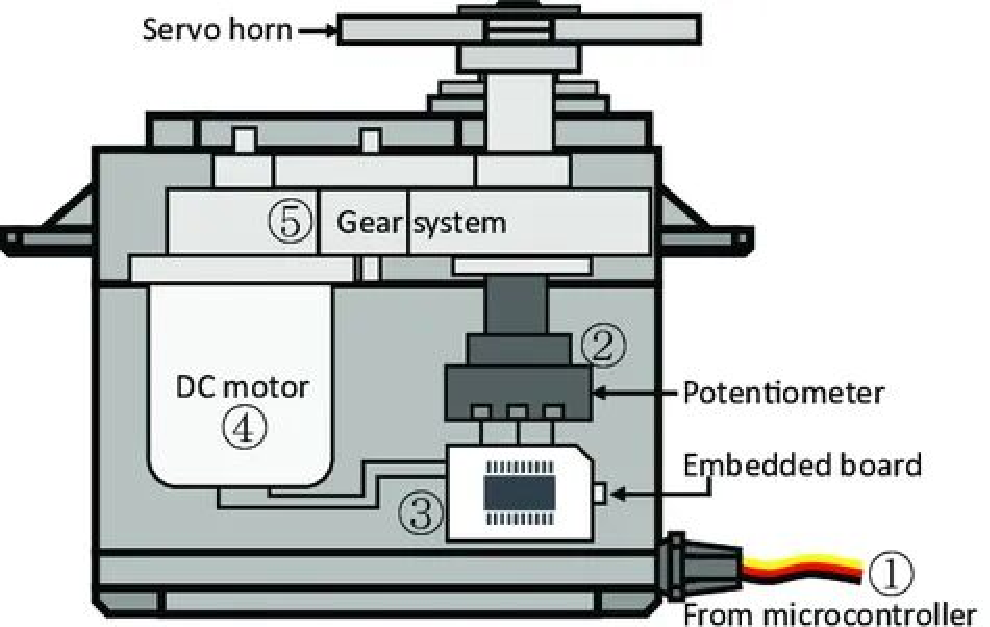
\includegraphics[width=0.8\textwidth]{images/servo_internal.pdf}
\floatnotes{}
%\label{fig:}
\caption{Servo Funktion}
\end{figure}

\hypertarget{grundlegende-eigenschaften}{%
\subsubsection{Grundlegende
Eigenschaften}\label{grundlegende-eigenschaften}}

\begin{itemize}

\item
  Ein Servo ist ein Motor, spezialisiert auf präzise Steuerung von
  Winkelpositionen.
\item
  Ausgestattet mit brauner (GND), orangefarbener (PWM-Signalleitung) und
  roter Leitung (VCC für Spannungsversorgung).
\end{itemize}

\hypertarget{unterschiede-zu-herkuxf6mmlichen-motoren}{%
\subsubsection{Unterschiede zu herkömmlichen
Motoren}\label{unterschiede-zu-herkoemmlichen-motoren}}

\begin{itemize}

\item
  Fähigkeit, zu spezifischen Positionen zu bewegen und diese exakt zu
  halten.
\item
  Kombiniert Zahnräder, ein Potentiometer und eine Steuerschaltung für
  seine Funktionalität.
\item
  Einsatz in Anwendungen, die präzise Positionskontrolle erfordern.
\end{itemize}

\hypertarget{technische-spezifikationen-1}{%
\subsubsection{Technische
Spezifikationen}\label{technische-spezifikationen-1}}

\begin{itemize}

\item
  \textbf{Motortyp}: Kernmotor.
\item
  \textbf{Betriebsspannung}: 4,8 bis 6V DC.
\item
  \textbf{Stromverbrauch}: \textless=50mA bei 4,8V, \textless=60mA bei
  6V im Leerlauf.
\item
  \textbf{Blockierstrom}: \textless=550mA bei 4,8V, \textless=650mA bei
  6V.
\item
  \textbf{Drehmoment}: \textgreater=0,6 kgf x cm bei 4,8V,
  \textgreater=0,7 kgf x cm bei 6V (Nennwert); \textgreater=1,4 kgf x cm
  bei 4,8V, \textgreater=1,6 kgf x cm bei 6V (Maximalwert).
\item
  \textbf{Leerlaufdrehzahl}: \textless=0,14s/60° bei 4,8V;
  \textless=0,12s/60° bei 6V.
\item
  \textbf{Betriebs- und Lagerungstemperatur}: -10 bis +50°C bzw. -20°C
  bis +60°C.
\item
  \textbf{Feuchtigkeitsbereiche}: \textless= 90\%RH für Betrieb und
  Lagerung.
\item
  \textbf{Gewicht}: 10+/- 0,5g.
\item
  \textbf{Material}: ABS.
\item
  \textbf{Betriebswinkel}: 180°+/-10°.
\item
  \textbf{Mechanischer Begrenzungswinkel}: 360°.
\end{itemize}

\hypertarget{kgf-kilogrammkraft}{%
\subsubsection{kgf (Kilogrammkraft)}\label{kgf-kilogrammkraft}}

>>kgf x cm<< ist eine Einheit für Drehmoment, die
Kilogrammkraft-Zentimeter bedeutet. Diese Einheit wird verwendet, um
auszudrücken, wie viel Drehmoment, also die Kraft einer Drehbewegung,
von einem Motor ausgeübt werden kann.

\begin{itemize}

\item
  \textbf{kgf (Kilogrammkraft)}: Eine Krafteinheit, die der auf ein
  Kilogramm Masse auf der Erdoberfläche ausgeübten Gravitationskraft
  entspricht. Technisch gesehen entspricht 1 kgf etwa 9,81 Newton (N),
  der SI-Einheit der Kraft.
\item
  \textbf{cm (Zentimeter)}: Eine Längeneinheit im metrischen System, die
  1/100 eines Meters entspricht.
\end{itemize}

\hypertarget{drehmomentwerte-des-servos-in-newtonzentimeter-ncm}{%
\subsubsection{Drehmomentwerte des Servos in Newtonzentimeter
(Ncm)}\label{drehmomentwerte-des-servos-in-newtonzentimeter-ncm}}

\begin{lstlisting}[language=Python]
# Umrechnungsfaktor von kgf·cm in Ncm
umrechnungsfaktor_kgf_cm_zu_n_cm = 9.81

# Gegebene Drehmomentwerte in kgf·cm
drehmoment_nenn_48v_kgf_cm = 0.6
drehmoment_nenn_6v_kgf_cm = 0.7
drehmoment_max_48v_kgf_cm = 1.4
drehmoment_max_6v_kgf_cm = 1.6

# Umrechnung in Ncm
drehmoment_nenn_48v_n_cm = drehmoment_nenn_48v_kgf_cm * umrechnungsfaktor_kgf_cm_zu_n_cm
drehmoment_nenn_6v_n_cm = drehmoment_nenn_6v_kgf_cm * umrechnungsfaktor_kgf_cm_zu_n_cm
drehmoment_max_48v_n_cm = drehmoment_max_48v_kgf_cm * umrechnungsfaktor_kgf_cm_zu_n_cm
drehmoment_max_6v_n_cm = drehmoment_max_6v_kgf_cm * umrechnungsfaktor_kgf_cm_zu_n_cm

drehmoment_nenn_48v_n_cm, drehmoment_nenn_6v_n_cm, drehmoment_max_48v_n_cm, drehmoment_max_6v_n_cm
\end{lstlisting}

\begin{itemize}

\item
  Bei \textbf{4,8V Nennwert}: ≥0,6 kgf·cm entspricht etwa 5,89 Ncm.
\item
  Bei \textbf{6V Nennwert}: ≥0,7 kgf·cm entspricht etwa 6,87 Ncm.
\item
  Bei \textbf{4,8V Maximalwert}: ≥1,4 kgf·cm entspricht etwa 13,73 Ncm.
\item
  Bei \textbf{6V Maximalwert}: ≥1,6 kgf·cm entspricht etwa 15,70 Ncm.
\end{itemize}

Diese Werte verdeutlichen die Kraft, die der Servo bei unterschiedlichen
Spannungen ausüben kann, und zeigen, dass mit steigender Spannung das
Drehmoment des Servos zunimmt.

\hypertarget{tt-motor}{%
\subsection{TT-Motor}\label{tt-motor}}

\begin{figure}
\centering
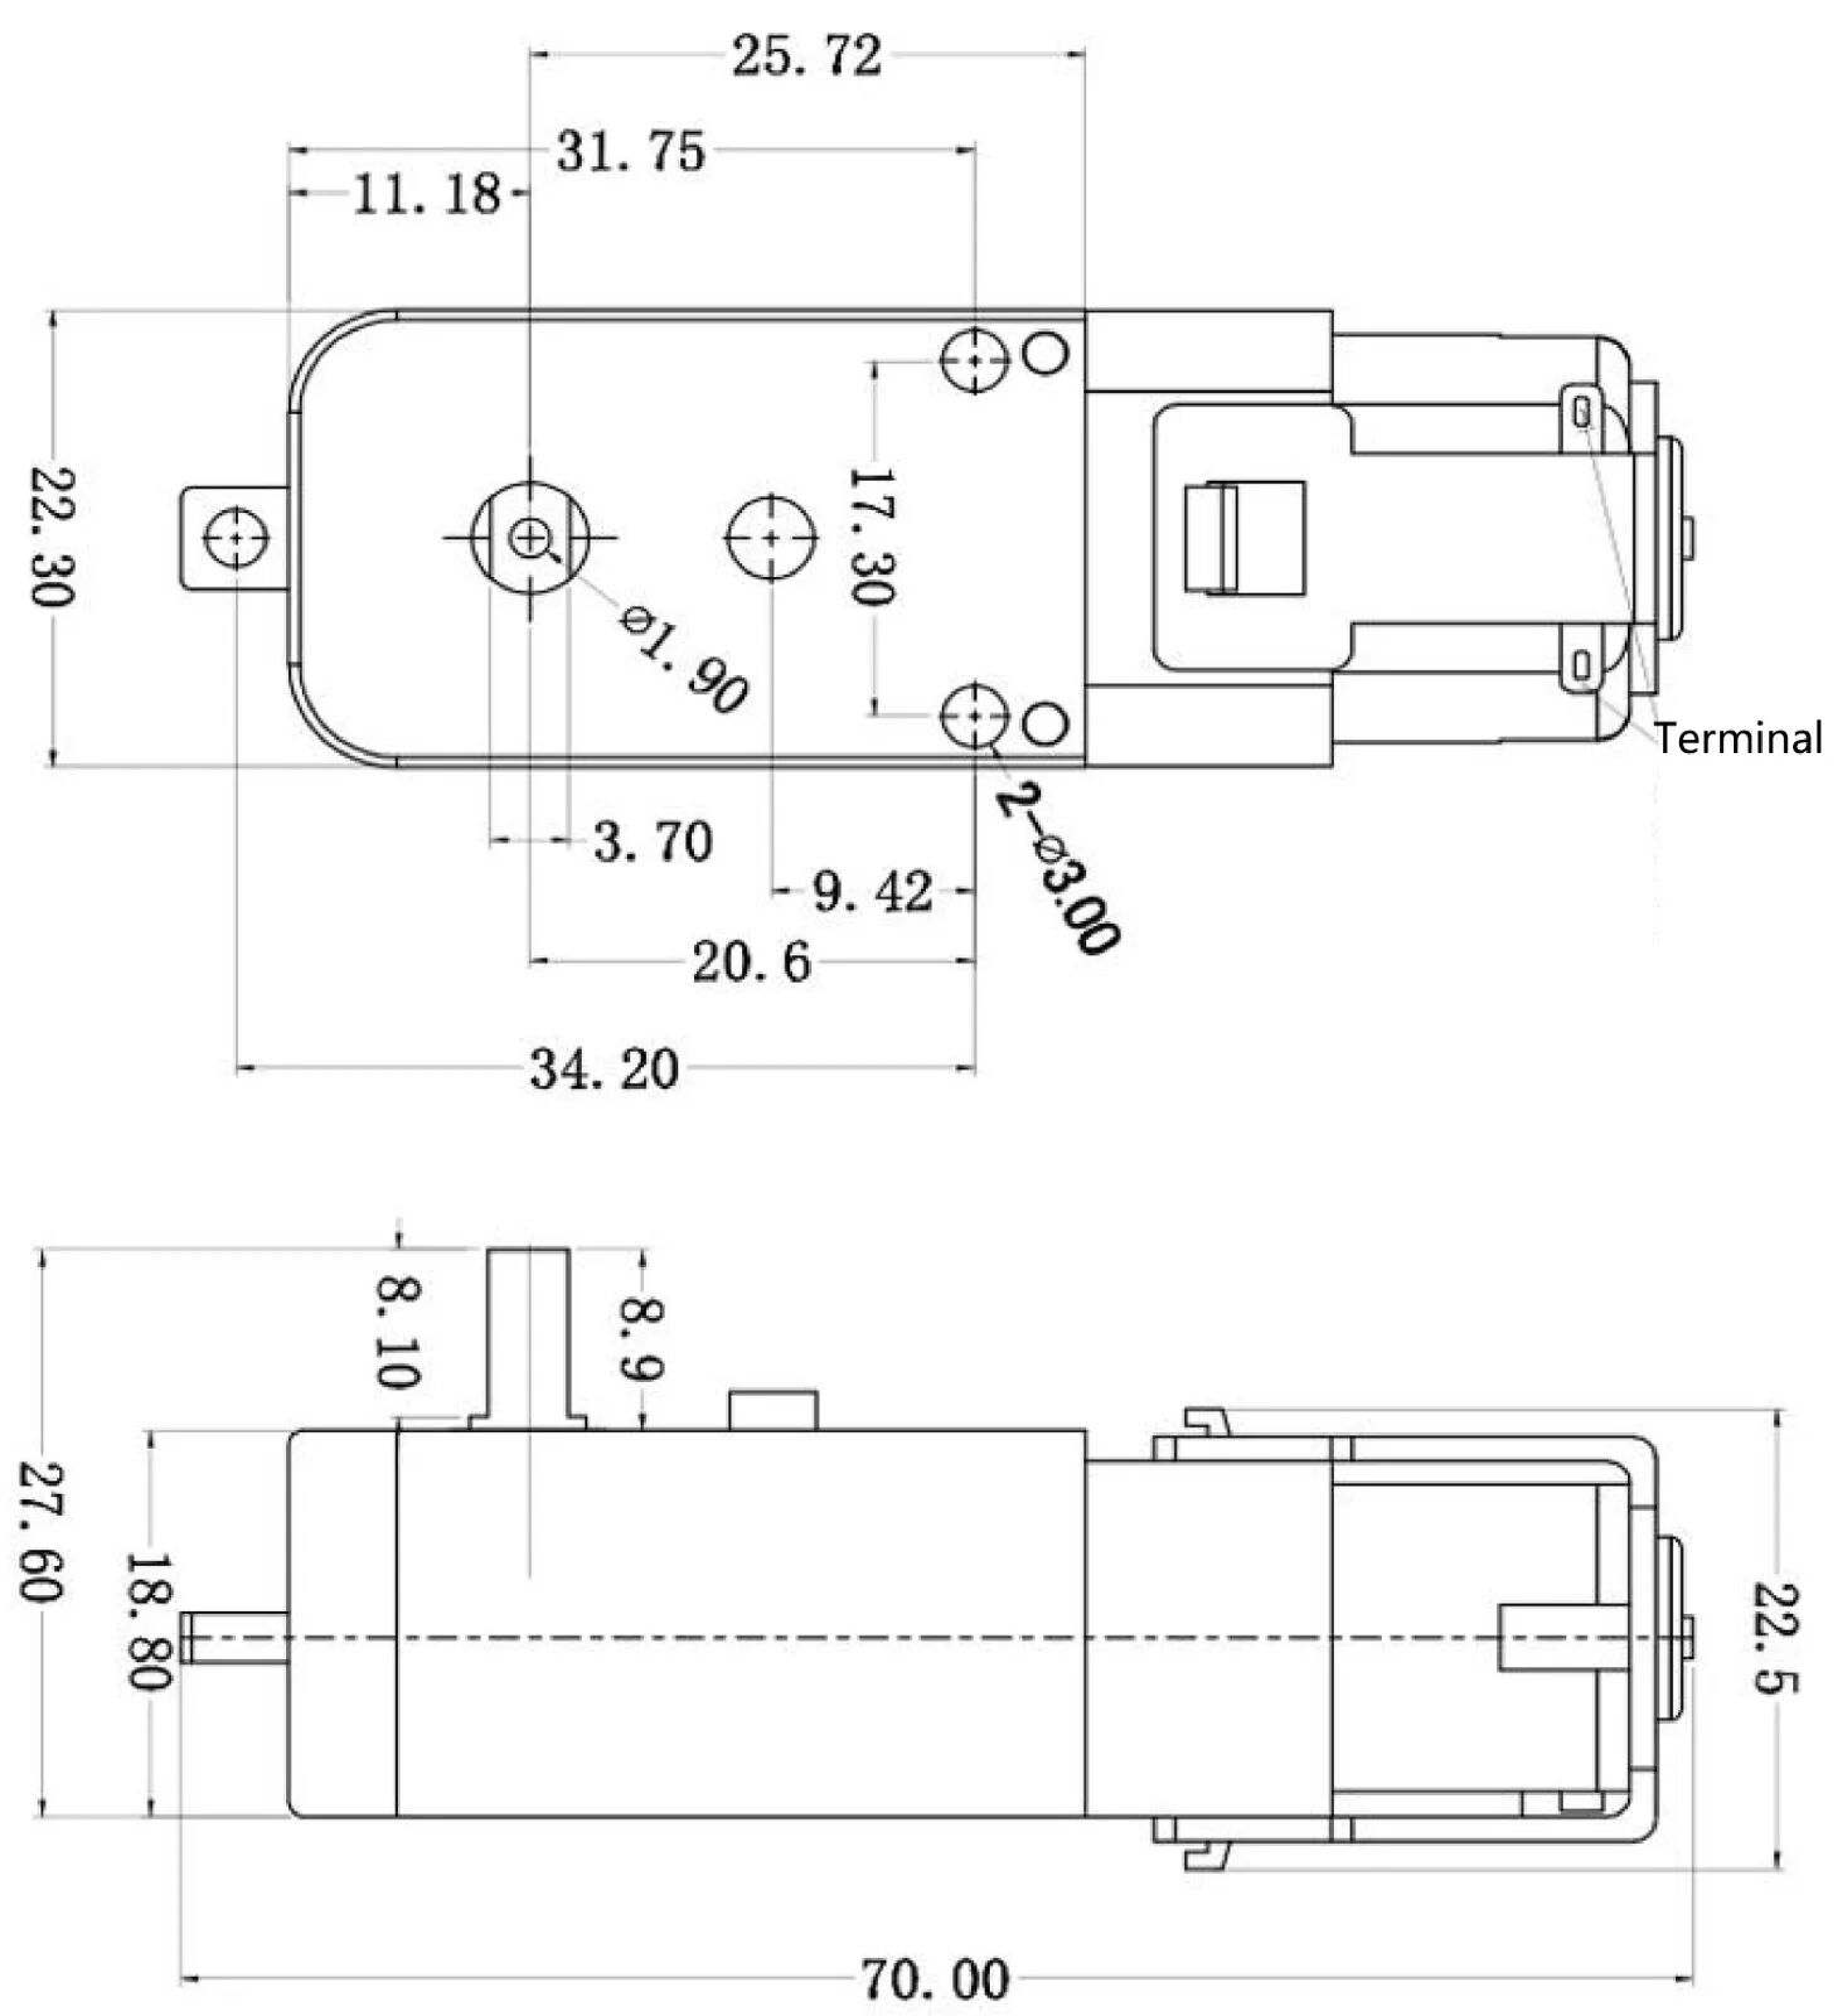
\includegraphics[width=0.8\textwidth]{images/motor_size.pdf}
\floatnotes{}
%\label{fig:}
\caption{Motor}
\end{figure}

\begin{figure}
\centering
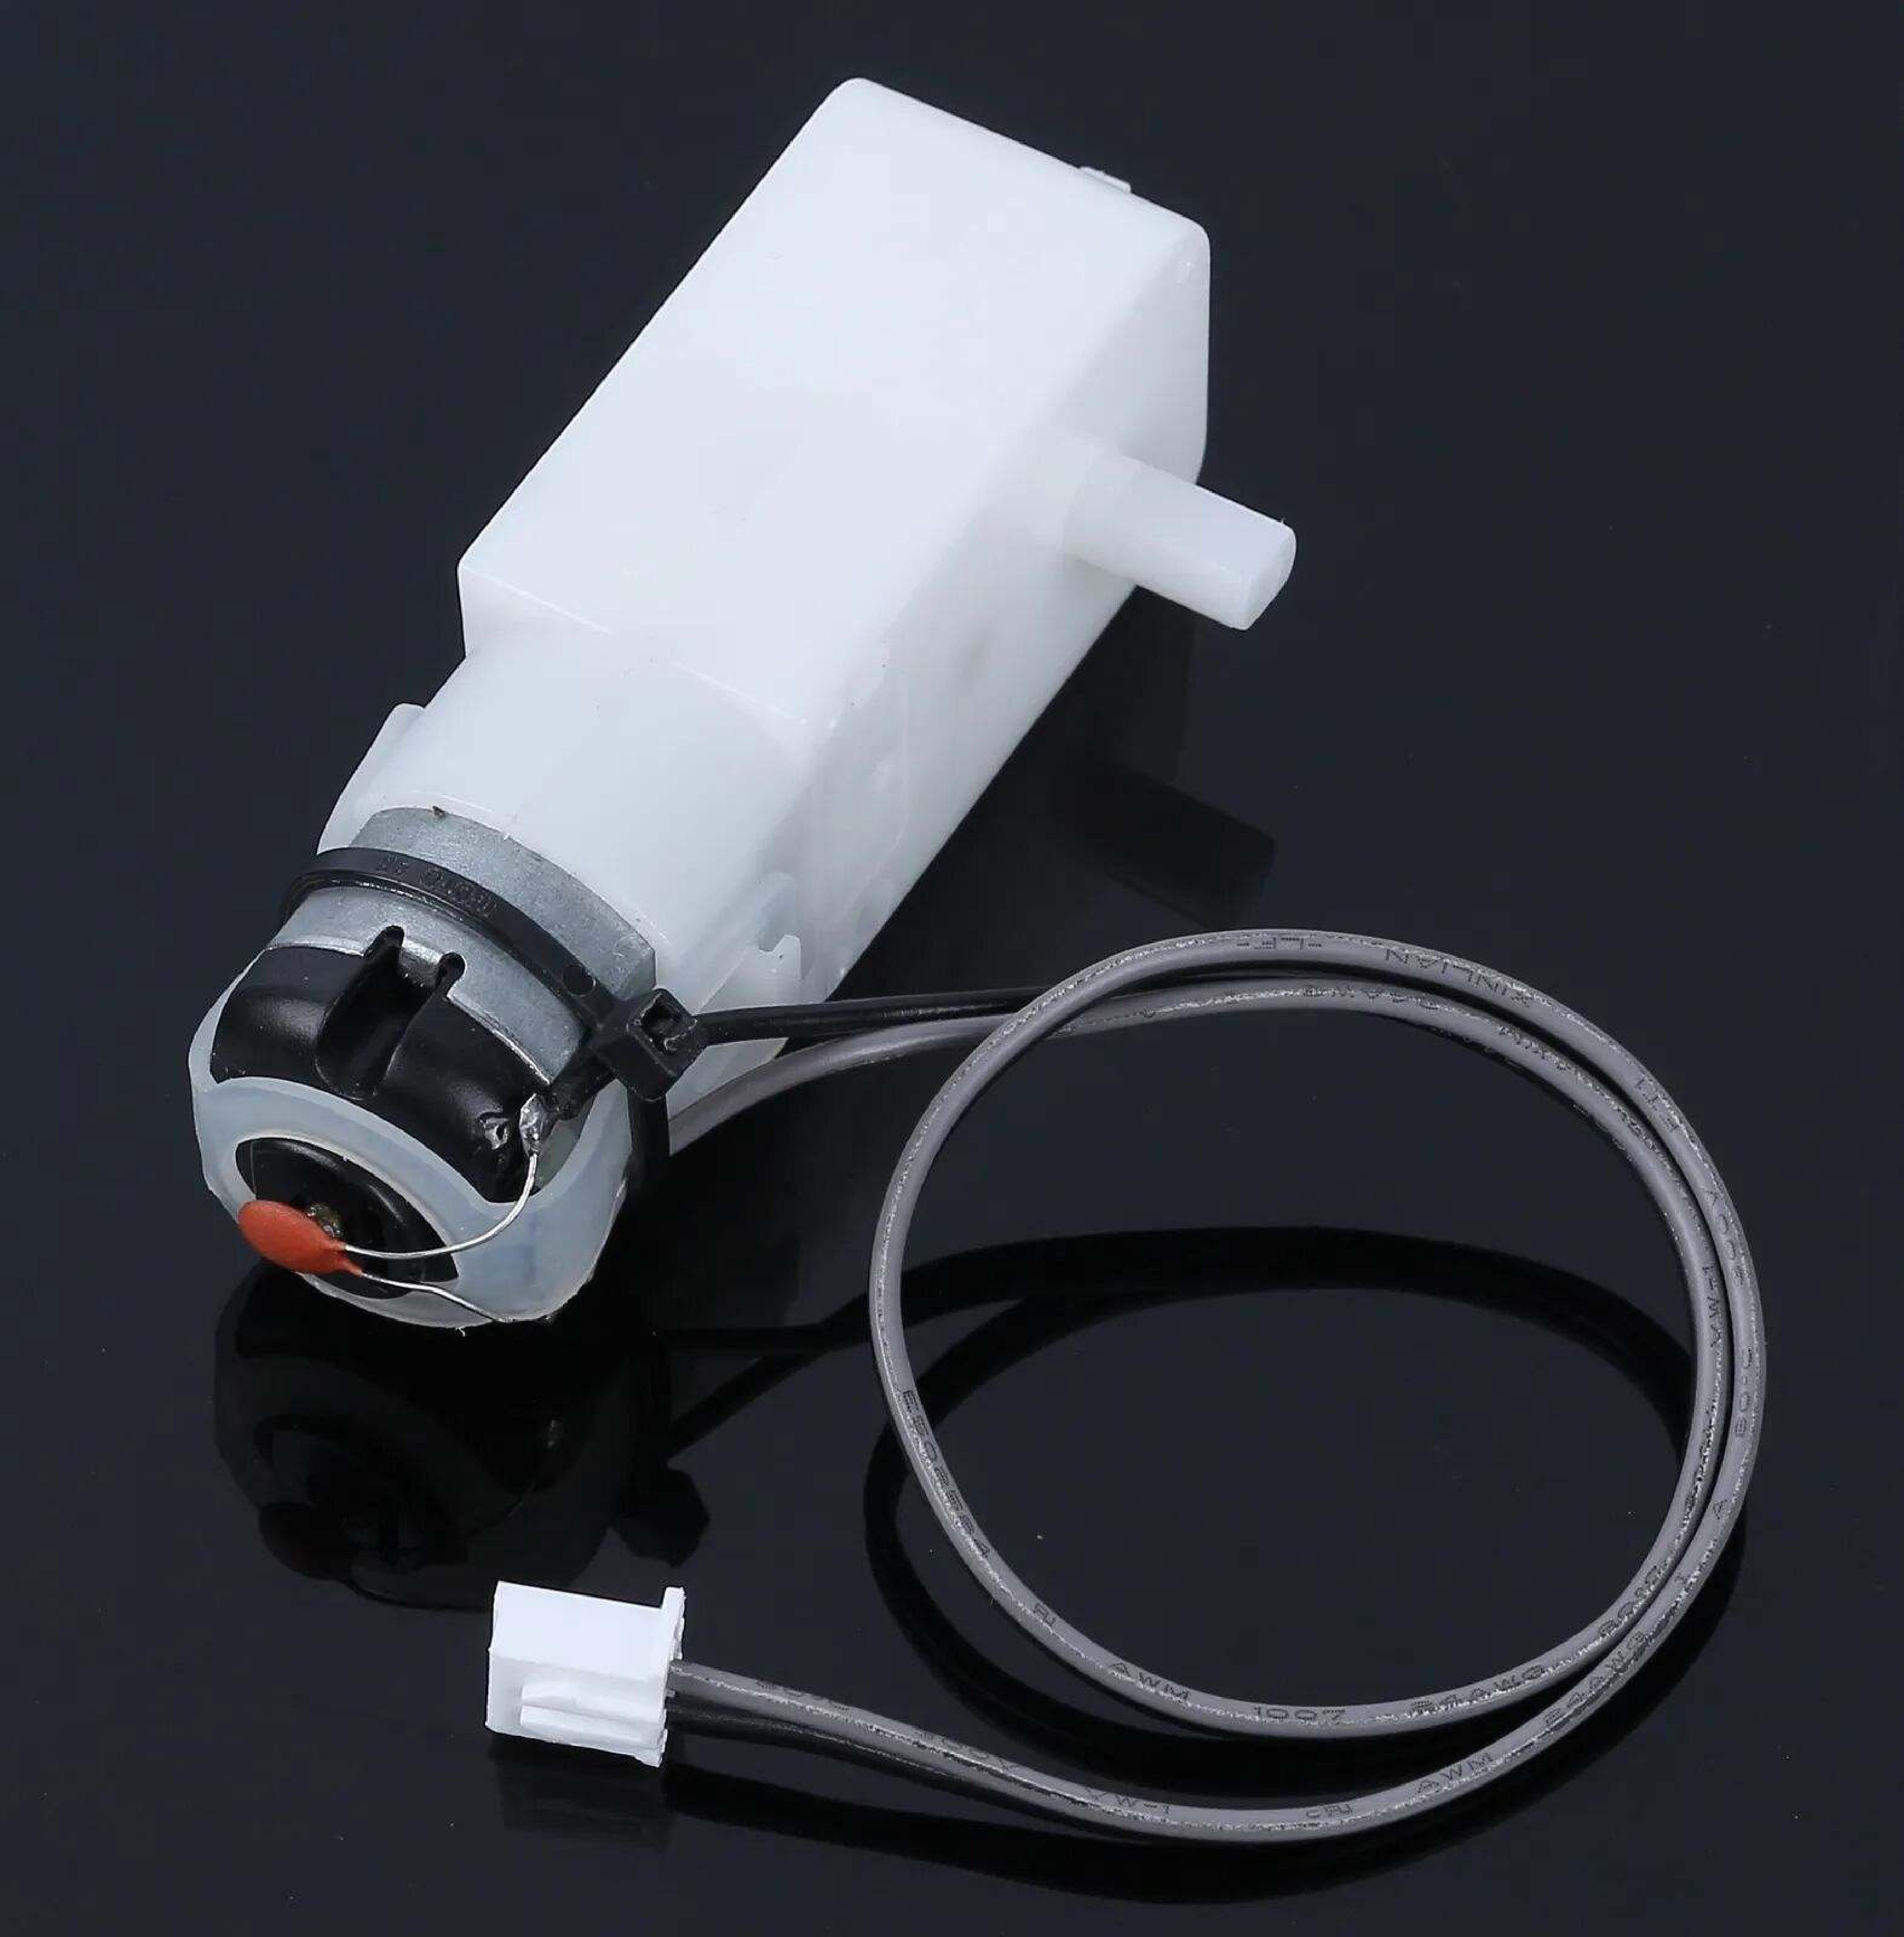
\includegraphics[width=0.8\textwidth]{images/tt_motor_xh.pdf}
\floatnotes{}
%\label{fig:}
\caption{TT-Getriebemotor}
\end{figure}

\hypertarget{beschreibung}{%
\subsubsection{Beschreibung}\label{beschreibung}}

\begin{itemize}

\item
  Der TT-DC-Getriebemotor ist mit einem Übersetzungsverhältnis von 1:120
  ausgestattet und für den Betrieb mit 3VDC konzipiert.
\item
  Ausgeliefert wird der Motor mit zwei 250 mm langen Kabeln, die über
  einen XH2.54-2P-Stecker verfügen.
\end{itemize}

\hypertarget{funktionsweise-von-motoren}{%
\subsubsection{Funktionsweise von
Motoren}\label{funktionsweise-von-motoren}}

\begin{itemize}

\item
  Motoren wandeln elektrische in mechanische Energie um
\item
  Ein Strom erzeugt ein Magnetfeld, das mit anderen Magneten interagiert
  und den Motor in Rotation versetzt.
\item
  Diese Drehbewegung kann dann auf Räder übertragen werden.
\end{itemize}

\hypertarget{spezifikationen-des-tt-getriebemotors}{%
\subsubsection{Spezifikationen des
TT-Getriebemotors}\label{spezifikationen-des-tt-getriebemotors}}

\begin{itemize}

\item
  \textbf{Spannungsbereich}: 3V bis 4.5V DC.
\item
  \textbf{Anzahl der Wellen}: Einzelwelle.
\item
  \textbf{Übersetzungsverhältnis}: 1:120.
\item
  \textbf{Leerlaufstrom}: 130mA.
\item
  \textbf{Leerlaufgeschwindigkeit}: 38rpm+/-8\%rpm.
\item
  \textbf{Startspannung}: Mindestens 2V im Leerlauf.
\item
  \textbf{Ausgangsdrehmoment}: Bei 3V über 1.2kgf x cm.
\item
  \textbf{Lebensdauer}: Zwischen 70 und 120 Stunden.
\item
  \textbf{Drehrichtung}: Kann in beide Richtungen drehen.
\item
  \textbf{Körperabmessungen}: 70 x 22,5 x 36,6mm.
\item
  \textbf{Kabel}: Grau und Schwarz, 24AWG, 250mm Länge.
\item
  \textbf{Stecker}: Weiß, XH2.54-2P.
\item
  \textbf{Gewicht}: 28,5g.
\end{itemize}

\hypertarget{gesamtdrehmoment-berechnen}{%
\subsubsection{Gesamtdrehmoment
berechnen}\label{gesamtdrehmoment-berechnen}}

Um das Gesamtdrehmoment in Newtonzentimeter (Ncm) zu berechnen, das von
sechs TT-DC-Getriebemotoren auf einem Marsrover bei einer Spannung von
3V erzeugt wird, wenn jedes einzelne Motor ein Ausgangsdrehmoment von
über 1.2 kgf·cm liefert.

\begin{enumerate}
\def\labelenumi{\arabic{enumi}.}

\item
  \textbf{Umrechnung von kgf·cm in Ncm}:

  \begin{itemize}
  
  \item
    Da 1 kgf etwa 9.81 N, entspricht 1 kgf x cm somit 9.81 Ncm.
  \end{itemize}
\item
  \textbf{Berechnung des Drehmoments pro Motor in Ncm}:

  \begin{itemize}
  
  \item
    $1.2 \, \text{kgf·cm} \times 9.81 \, \text{Ncm/kgf·cm} = 11.772 \, \text{Ncm}$
  \end{itemize}
\item
  \textbf{Gesamtdrehmoment für sechs Motoren}:

  \begin{itemize}
  
  \item
    $11.772 \, \text{Ncm} \times 6 = 70.632 \, \text{Ncm}$
  \end{itemize}
\end{enumerate}

\begin{lstlisting}[language=Python]
# Umrechnung von kgf·cm in Ncm für ein Drehmoment von 1.2 kgf·cm
drehmoment_pro_motor_kgf_cm = 1.2
umrechnungsfaktor_kgf_cm_zu_n_cm = 9.81  # 1 kgf·cm entspricht 9.81 Ncm

# Berechnung des Drehmoments pro Motor in Ncm
drehmoment_pro_motor_n_cm = drehmoment_pro_motor_kgf_cm * umrechnungsfaktor_kgf_cm_zu_n_cm

# Gesamtdrehmoment für sechs Motoren in Ncm
gesamtdrehmoment_n_cm = drehmoment_pro_motor_n_cm * 6

gesamtdrehmoment_n_cm
\end{lstlisting}

Das Gesamtdrehmoment, das von den sechs TT-DC-Getriebemotoren auf einem
Marsrover bei einer Spannung von 3V erzeugt wird, beträgt etwa 70.632
Ncm (Newtonzentimeter).

Dieses Drehmoment ermöglicht dem Rover, effektiv Bewegungen und Aktionen
auf der Marsoberfläche durchzuführen, wie das Überwinden von
Hindernissen oder das Manövrieren in schwierigem Gelände, indem es eine
starke und präzise Kraftübertragung auf die Räder oder andere
mechanische Komponenten bietet.

\hypertarget{solarpanel}{%
\subsection{Solarpanel}\label{solarpanel}}

\begin{figure}
\centering
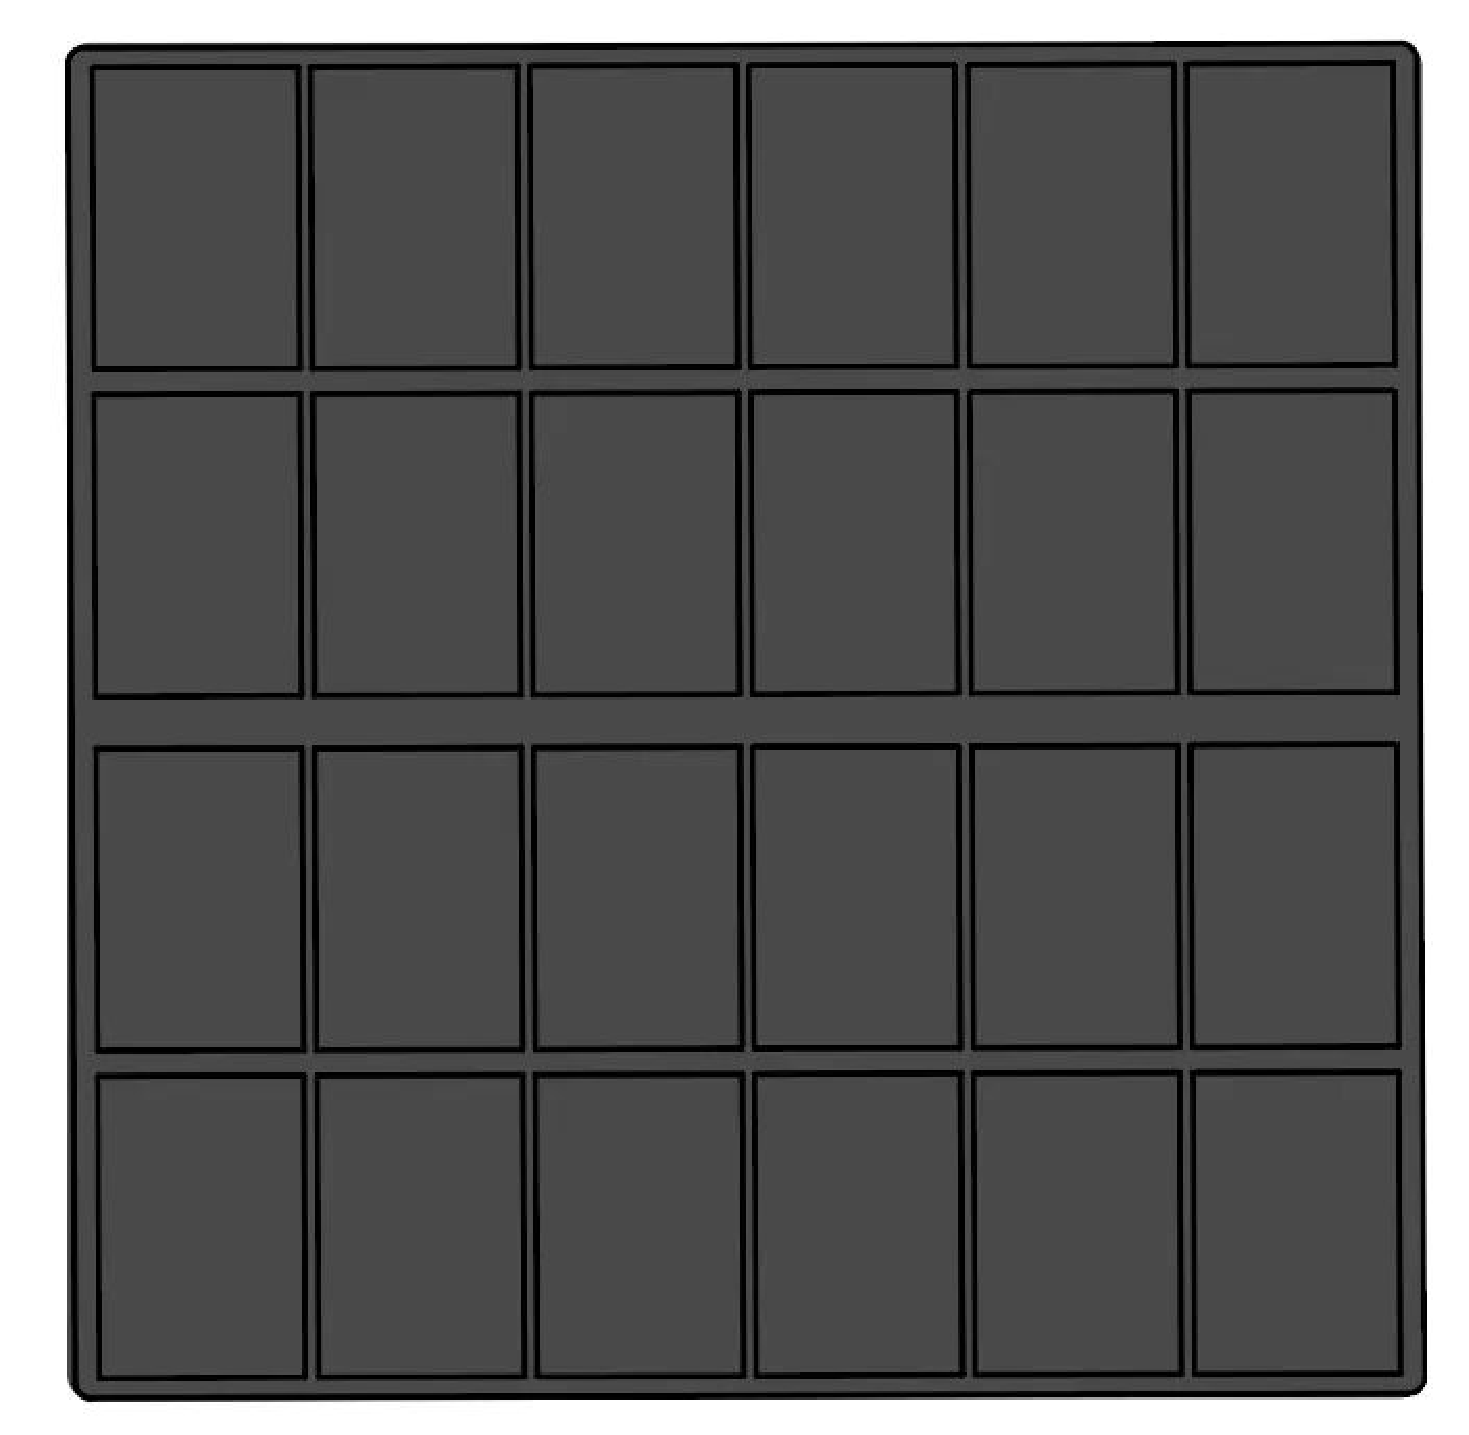
\includegraphics[width=0.8\textwidth]{images/solar_panel.pdf}
\floatnotes{}
%\label{fig:}
\caption{Solarpanel}
\end{figure}

Solarpanele wandeln Lichtenergie der Sonne in elektrische Energie um.

\begin{itemize}
\item
  \textbf{Funktionsweise}: Solarpanele bestehen aus photovoltaischen
  Zellen, häufig aus Silizium. Diese Zellen wandeln Sonnenlicht direkt
  in Elektrizität um. Wenn Sonnenlicht auf die Zellen trifft, werden
  Elektronen freigesetzt, die durch das Material fließen und so einen
  elektrischen Strom erzeugen.
\item
  \textbf{Merkmale eines Solarpanels}:

  \begin{itemize}
  
  \item
    \textbf{Ausgangsleistung}: 6V/660mA, was die Energiemenge angibt,
    die das Panel unter optimalen Bedingungen erzeugen kann.
  \item
    \textbf{Ladezeit}: Es benötigt theoretisch 7,2 Stunden unter starkem
    Sonnenlicht, um einen Akku vollständig aufzuladen. Diese Zeit kann
    als Richtwert für die Effizienz des Panels dienen.
  \item
    \textbf{Größe}: Mit Abmessungen von 170mm x 170mm ist es kompakt und
    vielseitig einsetzbar.
  \item
    \textbf{Kabel und Stecker}: Ausgestattet mit einem grauen und
    schwarzen Kabel (200mm lang, 24AWG) und einem weißen XH2.54-2P
    Stecker, was die Installation und Verbindung erleichtert.
  \end{itemize}
\end{itemize}

\hypertarget{rechenbeispiel-unter-verschiedenen-lichtverhuxe4ltnissen}{%
\subsubsection{Rechenbeispiel unter verschiedenen
Lichtverhältnissen}\label{rechenbeispiel-unter-verschiedenen-lichtverhaeltnissen}}

Um die Auswirkungen verschiedener Lichtverhältnisse auf Solarpanels zu
illustrieren, nehmen wir an, dass ein Solarpanel unter optimalen
Bedingungen (starkes Sonnenlicht) eine Ausgangsleistung von 6V/660mA
liefert und einen Akku in 7,2 Stunden vollständig aufladen kann.

\begin{enumerate}
\def\labelenumi{\arabic{enumi}.}

\item
  \textbf{Starkes Sonnenlicht}:

  \begin{itemize}
  
  \item
    Ausgangsleistung: 6V/660mA
  \item
    Ladezeit: 7,2 Stunden
  \end{itemize}
\item
  \textbf{Schwaches Sonnenlicht} (angenommen 50\% der optimalen
  Bedingungen):

  \begin{itemize}
  
  \item
    Ausgangsleistung wird halbiert: 6V/330mA (0,33A)
  \item
    Ladezeit verdoppelt sich theoretisch: 14,4 Stunden
  \end{itemize}
\item
  \textbf{Bewölkt} (angenommen 25\% der optimalen Bedingungen):

  \begin{itemize}
  
  \item
    Ausgangsleistung wird auf ein Viertel reduziert: 6V/165mA (0,165A)
  \item
    Ladezeit vervierfacht sich theoretisch: 28,8 Stunden
  \end{itemize}
\item
  \textbf{Nacht}:

  \begin{itemize}
  
  \item
    Keine Ausgangsleistung, da keine Sonneneinstrahlung vorhanden ist:
    0mA (0A)
  \item
    Keine Aufladung möglich
  \end{itemize}
\end{enumerate}

\hypertarget{auswirkungen}{%
\subsubsection{Auswirkungen}\label{auswirkungen}}

\begin{itemize}

\item
  \textbf{Starkes Sonnenlicht} ermöglicht die maximale Effizienz des
  Solarpanels, wodurch der Akku in der kürzesten Zeit aufgeladen wird.
\item
  \textbf{Schwaches Sonnenlicht} und \textbf{bewölkte Bedingungen}
  reduzieren die Ausgangsleistung des Panels, was zu einer verlängerten
  Ladezeit führt.
\item
  \textbf{Nacht} ist keine Aufladung möglich, da das Solarpanel auf die
  Umwandlung von Sonnenlicht in elektrische Energie angewiesen ist.
\end{itemize}

\hypertarget{batterie}{%
\subsection{18650 Batterie}\label{batterie}}

\begin{figure}
\centering
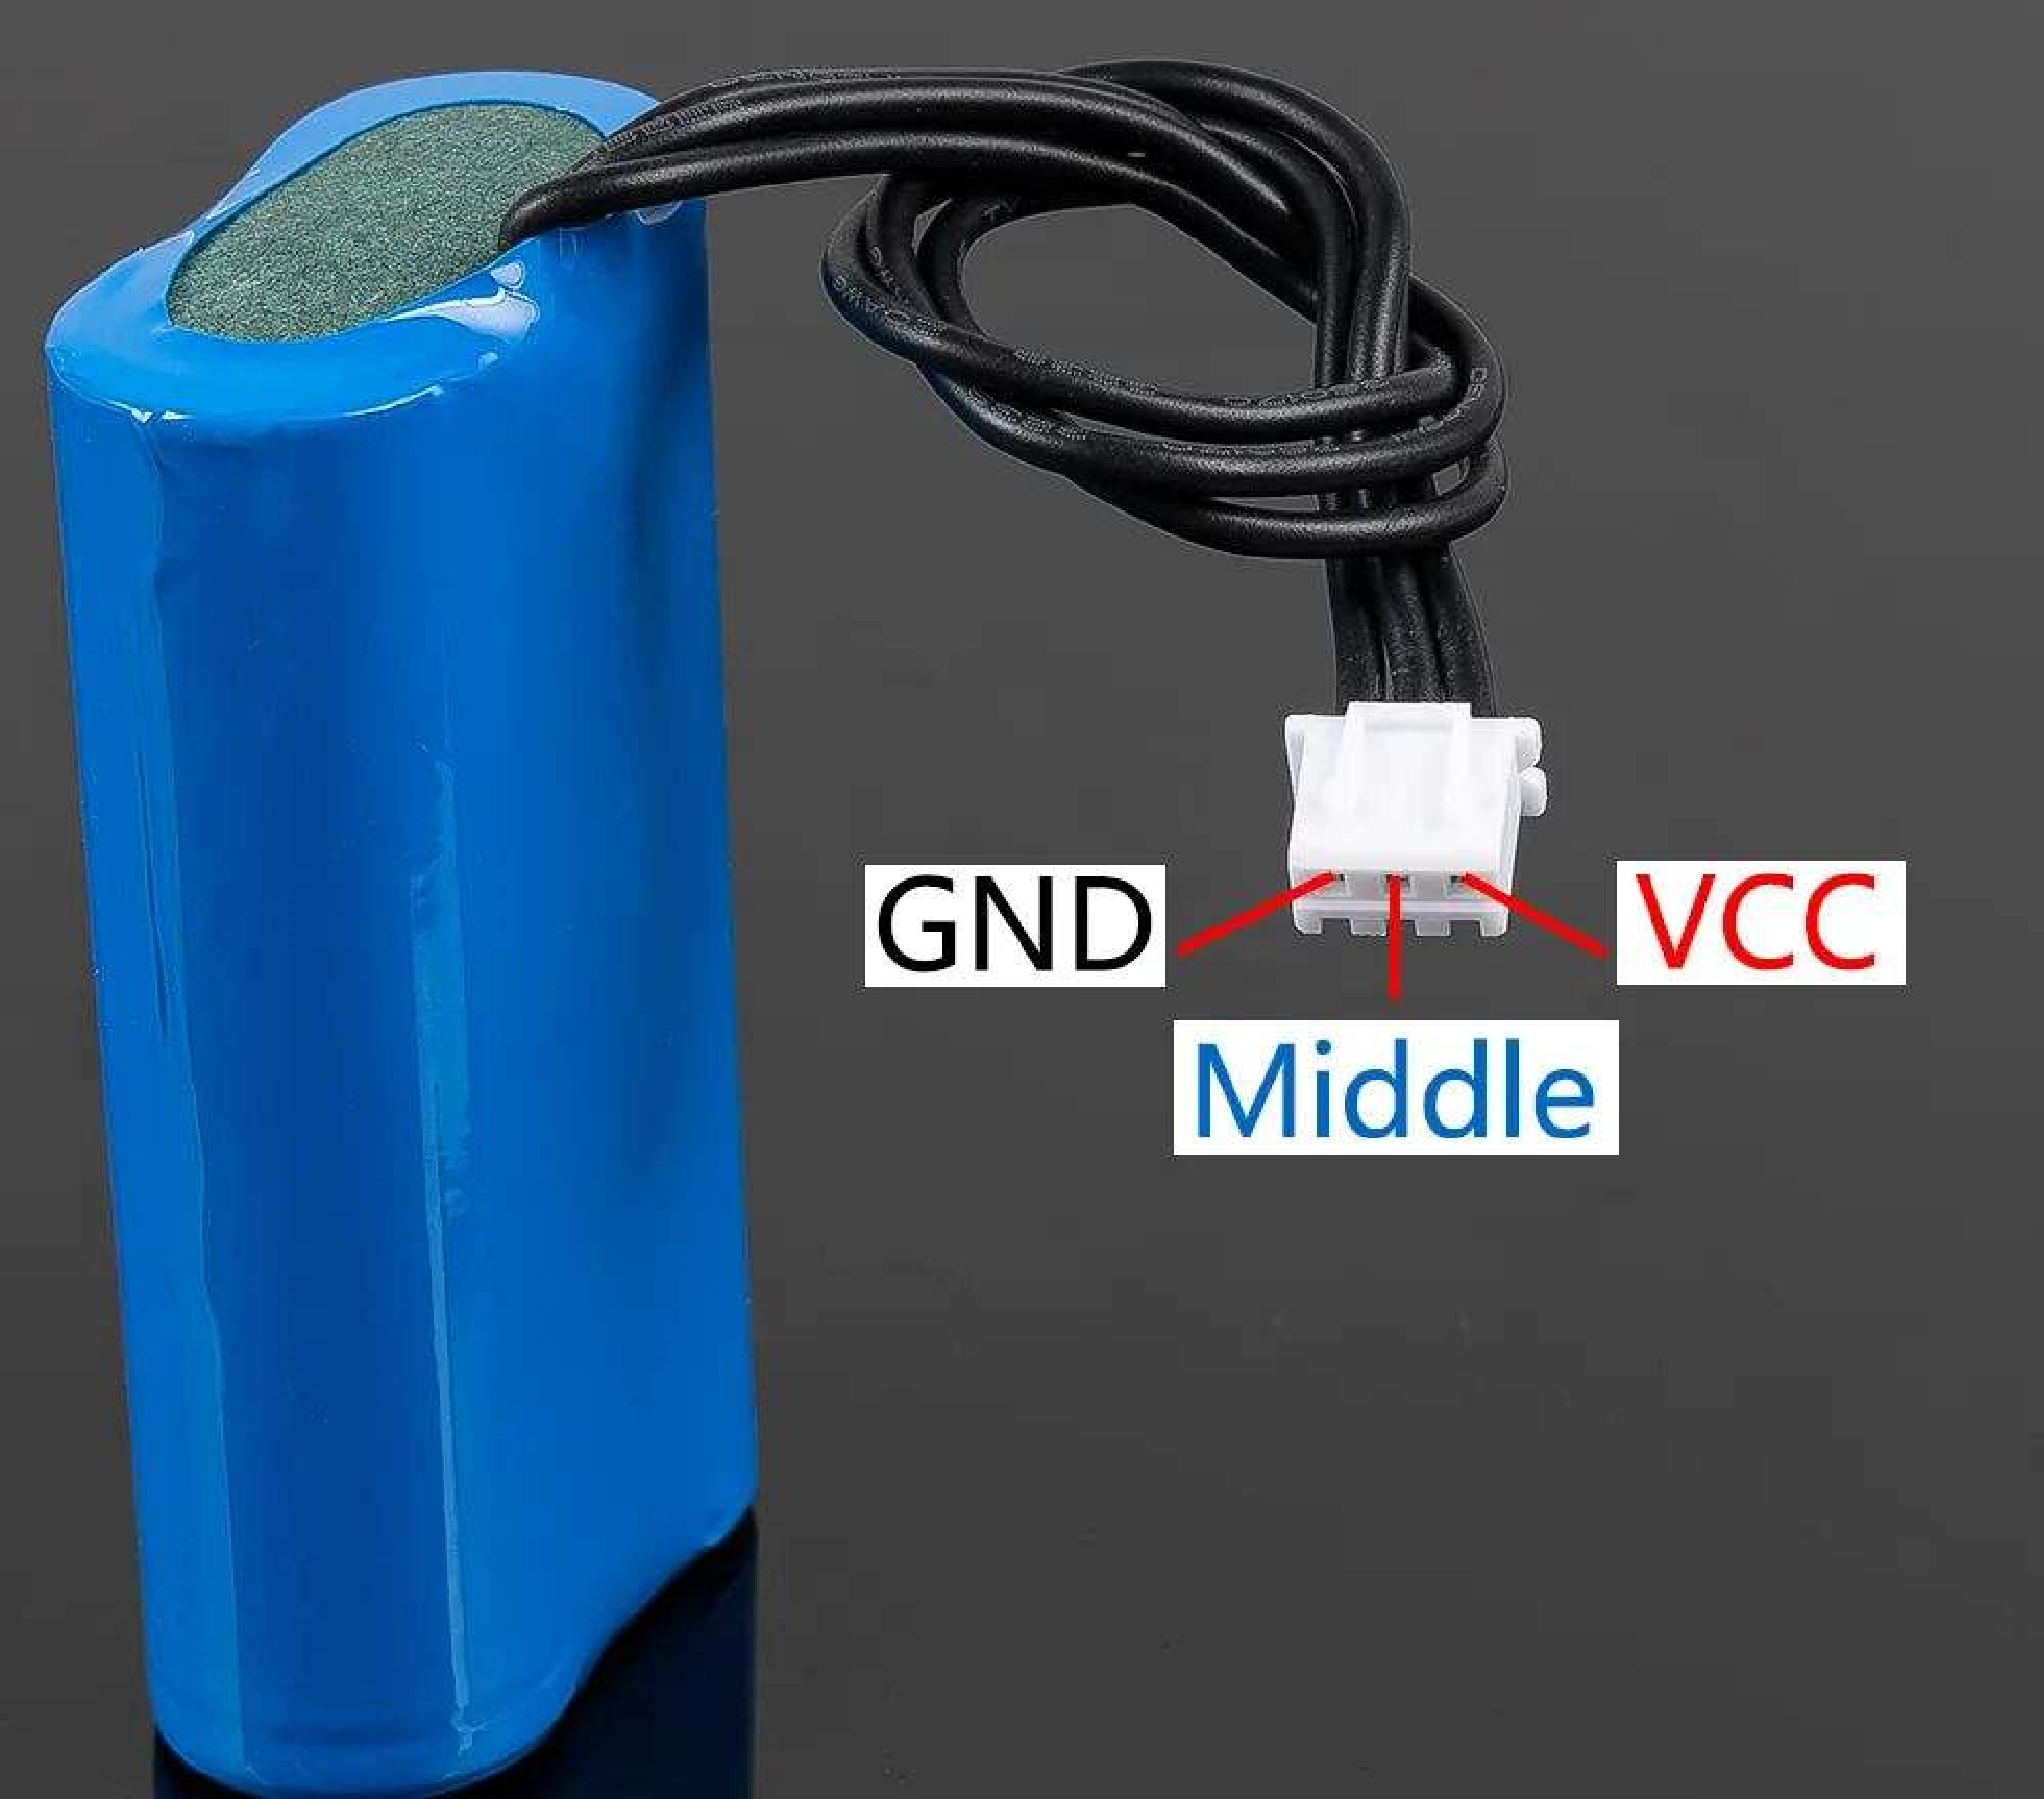
\includegraphics[width=0.8\textwidth]{images/3pin_battery.pdf}
\floatnotes{}
%\label{fig:}
\caption{3-Pin 18650 Batterie}
\end{figure}

\begin{itemize}

\item
  \textbf{Aufbau}: Das Batteriepaket besteht aus zwei 18650 Zellen mit
  jeweils einer Kapazität von 2000mAh, was eine Gesamtkapazität von
  4000mAh ergibt.
\item
  \textbf{Anschlüsse}:

  \begin{itemize}
  
  \item
    \textbf{VCC}: Positive Anschlüsse, vorhanden in zwei Sätzen, um den
    Stromfluss zu erhöhen und den Widerstand zu minimieren.
  \item
    \textbf{Middle}: Dient der Spannungsausgleichung zwischen den
    Zellen, um die Batterie zu schützen.
  \item
    \textbf{GND}: Negative Anschlüsse für den Stromkreis.
  \end{itemize}
\item
  \textbf{Anschlussart}: Verwendet wird ein XH2.54 3P-Anschluss, der
  eine direkte Aufladung des Batteriepakets ermöglicht, sobald es in ein
  kompatibles Shield eingesteckt wird.
\item
  \textbf{Leistung}:

  \begin{itemize}
  
  \item
    \textbf{Ladung}: Das Batteriepaket kann mit 5V/2A aufgeladen werden.
  \item
    \textbf{Ausgang}: Es liefert einen Ausgang von 5V/5A, geeignet für
    Anwendungen, die eine hohe Stromstärke benötigen.
  \end{itemize}
\item
  \textbf{Spezifikationen}:

  \begin{itemize}
  
  \item
    \textbf{Batteriekapazität}: Jede Zelle hat eine Kapazität von 3.7V
    und 2000mAh, insgesamt also 4000mAh bei Zusammenschaltung.
  \item
    \textbf{Batterielebensdauer}: Das Paket ermöglicht eine Laufzeit von
    etwa 90 Minuten bei voller Ladung.
  \item
    \textbf{Ladezeit}: Die vollständige Aufladung des Batteriepakets
    dauert ca. 130 Minuten.
  \end{itemize}
\end{itemize}

\hypertarget{ladeanschluss-charge-port}{%
\subsubsection{Ladeanschluss (Charge
Port)}\label{ladeanschluss-charge-port}}

\begin{itemize}

\item
  \textbf{Typ}: USB-C-Port mit 5V/2A für das Aufladen.
\item
  \textbf{Ladezeit}: Der Akku kann innerhalb von 130 Minuten vollständig
  aufgeladen werden.
\end{itemize}

\hypertarget{batterieanschluss-battery-port}{%
\subsubsection{Batterieanschluss (Battery
Port)}\label{batterieanschluss-battery-port}}

\begin{itemize}

\item
  \textbf{Spannungsbereich}: 6.6V bis 8.4V über einen
  PH2.0-3P-Stromversorgungseingang.
\end{itemize}

\hypertarget{solaranschluss}{%
\subsubsection{Solaranschluss}\label{solaranschluss}}

\begin{itemize}

\item
  \textbf{Funktion}: Ermöglicht das Aufladen des Akkus über ein
  Solarpanel.
\item
  \textbf{Anschlusstyp}: XH2.54, 2P.
\item
  \textbf{Ausgangsleistung des Solarpanels}: 6V/660mA.
\item
  \textbf{Ladezeit}: Unter starkem Sonnenlicht kann der Akku theoretisch
  in 7,2 Stunden vollständig aufgeladen werden.
\end{itemize}

\hypertarget{x18650-batterien-in-reihe}{%
\subsubsection{2x18650 Batterien in
Reihe}\label{x18650-batterien-in-reihe}}

\begin{itemize}

\item
  \textbf{Konfiguration}: Zwei 18650 Batterien, jede mit 3.7V und
  2000mAh.
\item
  \textbf{Schaltung in Reihe}: Durch die Reihenschaltung der beiden
  Batterien erhöht sich die Gesamtspannung auf 7.4V, während die
  Gesamtkapazität bei 2000mAh bleibt.
\end{itemize}

\hypertarget{ladezeit-berechnen}{%
\subsubsection{Ladezeit berechnen}\label{ladezeit-berechnen}}

Die Ladezeit eines Akkus hängt von seiner Kapazität (in
Milliamperestunden, mAh) und dem Ladestrom (in Ampere, A) ab.

$\text{Ladezeit (Stunden)} = \frac{\text{Kapazität des Akkus (mAh)}}{\text{Ladestrom (mA)}}$

Für zwei 18650 Batterien in Reihe geschaltet, mit jeweils 3.7V und
2000mAh, ergibt sich eine Gesamtspannung von 7.4V und eine Kapazität von
2000mAh (da die Kapazität in Reihe gleich bleibt). Der Ladestrom ist mit
2A (oder 2000mA) angegeben.

\begin{lstlisting}[language=Python]
# Gegebene Daten
kapazitaet_mAh = 2000  # Kapazität einer der 18650 Batterien in mAh
ladestrom_mA = 2000  # Ladestrom in mA (5V/2A)

# Berechnung der Ladezeit in Stunden
ladezeit_stunden = kapazitaet_mAh / ladestrom_mA

# Umrechnung der Ladezeit in Minuten
ladezeit_minuten = ladezeit_stunden * 60

ladezeit_minuten
\end{lstlisting}

Die berechnete Ladezeit für eine 18650 Batterie mit einer Kapazität von
2000mAh unter Verwendung eines Ladestroms von 2A (2000mA) beträgt 60
Minuten.

Die Angabe von 130 Minuten Ladezeit könnte auf eine konservativere
Schätzung hinweisen, die möglicherweise Effizienzverluste beim Laden
oder die Charakteristiken des spezifischen Ladesystems berücksichtigt.
Es könnte auch darauf hindeuten, dass der tatsächliche Ladestrom unter
bestimmten Umständen, wie zum Beispiel bei niedrigerer Spannung des
Ladegeräts oder bei internen Widerständen in der Batterieschaltung,
effektiv niedriger als 2A ist, was zu einer längeren Ladezeit führt.

\hypertarget{batterielebensdauer-und-entladestromstuxe4rke-berechnen}{%
\subsubsection{Batterielebensdauer und Entladestromstärke
berechnen}\label{batterielebensdauer-und-entladestromstaerke-berechnen}}

Wenn die Batterie 90 Minuten lang hält, können wir den
durchschnittlichen Entladestrom ($I$) berechnen, der für diese
Laufzeit benötigt wird, mit der Formel:

$I = \frac{\text{Kapazität}}{\text{Betriebsdauer in Stunden}}$

Um die Betriebsdauer in Stunden umzurechnen, teilen wir 90 Minuten durch
60:

$\text{Betriebsdauer} = \frac{90}{60} = 1,5 \, \text{Stunden}$

Daraus ergibt sich:

$I = \frac{2000 \, \text{mAh}}{1,5 \, \text{Stunden}} = \frac{2000}{1,5} \, \text{mA} = 1333,33 \, \text{mA}$

Dies bedeutet, dass das Gerät durchschnittlich etwa 1333,33 mA (oder
1,33 A) über die Dauer von 90 Minuten verbraucht, um die Batterie
vollständig zu entladen. % Platzhalter

%% Optional Anhang
%\clearpage
%\appendix

\clearpage
\printbibliography
\end{document}